% TEX file generated by R with the 'knitr' package
%
% DO NOT EDIT THE TEX FILE DIRECTLY
% ===========================================================================================================

\documentclass[a4paper, notitlepage]{extreport}\usepackage[]{graphicx}\usepackage{xcolor}
% maxwidth is the original width if it is less than linewidth
% otherwise use linewidth (to make sure the graphics do not exceed the margin)
\makeatletter
\def\maxwidth{ %
  \ifdim\Gin@nat@width>\linewidth
    \linewidth
  \else
    \Gin@nat@width
  \fi
}
\makeatother

\definecolor{fgcolor}{rgb}{0.345, 0.345, 0.345}
\newcommand{\hlnum}[1]{\textcolor[rgb]{0.686,0.059,0.569}{#1}}%
\newcommand{\hlstr}[1]{\textcolor[rgb]{0.192,0.494,0.8}{#1}}%
\newcommand{\hlcom}[1]{\textcolor[rgb]{0.678,0.584,0.686}{\textit{#1}}}%
\newcommand{\hlopt}[1]{\textcolor[rgb]{0,0,0}{#1}}%
\newcommand{\hlstd}[1]{\textcolor[rgb]{0.345,0.345,0.345}{#1}}%
\newcommand{\hlkwa}[1]{\textcolor[rgb]{0.161,0.373,0.58}{\textbf{#1}}}%
\newcommand{\hlkwb}[1]{\textcolor[rgb]{0.69,0.353,0.396}{#1}}%
\newcommand{\hlkwc}[1]{\textcolor[rgb]{0.333,0.667,0.333}{#1}}%
\newcommand{\hlkwd}[1]{\textcolor[rgb]{0.737,0.353,0.396}{\textbf{#1}}}%
\let\hlipl\hlkwb

\usepackage{framed}
\makeatletter
\newenvironment{kframe}{%
 \def\at@end@of@kframe{}%
 \ifinner\ifhmode%
  \def\at@end@of@kframe{\end{minipage}}%
  \begin{minipage}{\columnwidth}%
 \fi\fi%
 \def\FrameCommand##1{\hskip\@totalleftmargin \hskip-\fboxsep
 \colorbox{shadecolor}{##1}\hskip-\fboxsep
     % There is no \\@totalrightmargin, so:
     \hskip-\linewidth \hskip-\@totalleftmargin \hskip\columnwidth}%
 \MakeFramed {\advance\hsize-\width
   \@totalleftmargin\z@ \linewidth\hsize
   \@setminipage}}%
 {\par\unskip\endMakeFramed%
 \at@end@of@kframe}
\makeatother

\definecolor{shadecolor}{rgb}{.97, .97, .97}
\definecolor{messagecolor}{rgb}{0, 0, 0}
\definecolor{warningcolor}{rgb}{1, 0, 1}
\definecolor{errorcolor}{rgb}{1, 0, 0}
\newenvironment{knitrout}{}{} % an empty environment to be redefined in TeX

\usepackage{alltt}

% Captions in floating environments
\usepackage{titling}
\usepackage{authblk}
\usepackage{framed}
\usepackage{xcolor}
\usepackage{amsmath}
\usepackage{type1cm}
\usepackage{lettrine}
\usepackage{natbib}
\usepackage{pgfplots}
\pgfplotsset{compat=1.16}

% captions
\usepackage[font=footnotesize,
            labelfont=bf,
            textfont=it,
            margin=.5cm
            ]{caption}

%\setlength{\parskip}{1em}
\edef\restoreparindent{\parindent=\the\parindent\relax}
\usepackage{parskip}
\restoreparindent

% todo notes
\usepackage{todonotes}

% sans font
\usepackage[defaultsans]{droidsans}

% margins
\usepackage[a4paper,margin=2.5cm]{geometry}

\usepackage{setspace}
\onehalfspacing

% pagestyle
\usepackage{fancyhdr}
\usepackage{lastpage}

\fancypagestyle{newchapter}{%
\fancyhf{} % clear all header and footer fields
\renewcommand{\headrulewidth}{0pt}
\renewcommand{\footrulewidth}{0pt}
\rfoot{\ruleline{\fontsize{9}{9}\bfseries Page \thepage\ of \pageref{LastPage}}}
}

\fancypagestyle{firststyle}{
\fancyhf{}
\renewcommand{\headrulewidth}{0pt}
\setlength{\headsep}{10pt}
\renewcommand{\footrulewidth}{0pt}
\lhead{\rulelinel{\fontsize{9}{9}\bfseries \leftmark}}
\rfoot{\ruleline{\fontsize{9}{9}\bfseries Page \thepage\ of \pageref{LastPage}}}
\setlength{\footskip}{20pt}
}

\fancypagestyle{preamble}{
\fancyhf{}
\renewcommand{\headrulewidth}{0pt}
\lfoot{\rulelinel{\fontsize{9}{9}\bfseries \thepage}}
}

\fancypagestyle{ack}{
\fancyhf{}
\renewcommand{\headrulewidth}{0.4pt}
\lfoot{\rulelinel{\fontsize{9}{9}\bfseries \thepage}}
}

\fancypagestyle{empty}{
\fancyhf{}
\renewcommand{\headrulewidth}{.4pt}
\renewcommand{\footrulewidth}{.4pt}
}

% For subcaptions in figures
\usepackage{subcaption}

% For sidewaysfigure
%\usepackage{rotfloat}

% For professional looking tables
\usepackage{booktabs} 

%\usepackage{multirow}
\usepackage{multicol}
%\usepackage{longtable}
%\usepackage{tabularx}

% For \FloatBarrier
\usepackage[section,below]{placeins}

% Linebreaks in tables
\usepackage{makecell}
\usepackage{wrapfig}

% Hyperlinks
\definecolor{darkblue}{rgb}{0.0,0.0,0.4}
\definecolor{darkred}{rgb}{0.5,0.0,0.0}
\usepackage{hyperref}
\hypersetup{
    colorlinks = true,
    linkcolor = darkred,
    anchorcolor = darkred,
    citecolor = darkred,
    urlcolor = darkblue
}
\urlstyle{sf}
% main font
%\usepackage{XCharter} %% cf http://www.khirevich.com/latex/font/
\usepackage[bitstream-charter]{mathdesign}
% For underscores that correspond to the encoding
\usepackage[T1]{fontenc}

% Table of content settings
\setcounter{tocdepth}{2}
\setcounter{secnumdepth}{2}
\usepackage{tocbasic}
\addtotoclist[report.cls]{toc}
\renewcommand*{\tableofcontents}{\listoftoc[{\contentsname}]{toc}}% ToC under control of tocbasic
\AfterTOCHead[toc]{\thispagestyle{preamble}\pagestyle{ack}}
\AfterStartingTOC[toc]{\clearpage}

% Allowed percentages of page a float can use
\renewcommand{\textfraction}{0.05}
\renewcommand{\topfraction}{0.95}
\renewcommand{\bottomfraction}{0.95}
\renewcommand{\floatpagefraction}{0.75}

% Figure names
\renewcommand{\figurename}{Fig.}

% Used for knitr images from Rnw files
\newcommand{\subfloat}[2][default for first parameter: need a sub-caption]{\subcaptionbox{#1}{#2}}

% Typesetting commands
\newcommand{\R}{\textbf{\textsf{R}}}

%%% My additions %%%
\newcommand*\ruleline[1]{\par\noindent\raisebox{.8ex}{\makebox[\linewidth]{\hrulefill\hspace{1ex}\raisebox{-.6ex}{#1}\hspace{1ex}}}}

\newcommand*\rulelinel[1]{\par\noindent\raisebox{.8ex}{\makebox[\linewidth]{\hrulefill\hspace{1ex}\raisebox{-.6ex}{#1}\hspace{1ex}\hrulefill}}}

% change chapters
\usepackage{titlesec}

\titleformat{\chapter}
{\Large\bfseries}
{}
{0.5em}
{\titlerule\, \thechapter. \thispagestyle{newchapter}}

\titleformat{name=\chapter,numberless}
{\Large\bfseries}
{}
{0.5em}
{\titlerule\enspace \thispagestyle{preamble}}
[]

% sections
\titleformat{\section}
{\large\bfseries}
{}
{0.5em}
{\thesection. }
[]

\titleformat{name=\section,numberless}
{\large\bfseries}
{}
{0.5em}
{}
[]

% subsections
\titleformat{\subsection}
{\normalsize\itshape\bfseries}
{}
{0.5em}
{\thesubsection. }
[]

% subsections
\titleformat{\subsubsection}
{\small\itshape}
{}
{0.5em}
{\thesubsubsection. }
[]

\providecommand{\keywords}[1]{\footnotesize\textbf{\textit{Keywords:}} #1}

\newcommand{\copyrightfont}{\linespread{1}\normalfont\rmfamily\fontsize{7}{8}\selectfont}
\newcommand{\ackfont}{\rmfamily\bfseries\fontsize{9}{9}\selectfont}
\renewcommand\Authfont{\normalfont\sffamily\bfseries\fontsize{11}{11}\selectfont}
\newcommand{\datesfont}{\linespread{1}\normalfont\sffamily\fontsize{10}{8}\selectfont}
\newcommand{\titlefont}{\linespread{1}\normalfont\rmfamily\fontsize{22pt}{24pt}\selectfont}

% bib
\setlength{\bibsep}{10pt}
\renewcommand*{\bibfont}{\normalfont\rmfamily\fontsize{9.5}{10}\selectfont} % set font to be sans serif

\pagestyle{firststyle}

\renewcommand*\footnoterule{}

\usepackage{multicol}
\usepackage{etoolbox}
\usepackage{relsize}
\patchcmd{\thebibliography}
  {\list}
  {\begin{multicols}{2}\smaller\list}
  {}
  {}
\appto{\endthebibliography}{\end{multicols}}

\appto\appendix{\addtocontents{toc}{\protect\setcounter{tocdepth}{1}}}

% reinstate the correct level for list of tables and figures
\appto\listoffigures{\addtocontents{lof}{\protect\setcounter{tocdepth}{1}}}
\appto\listoftables{\addtocontents{lot}{\protect\setcounter{tocdepth}{1}}}

\IfFileExists{upquote.sty}{\usepackage{upquote}}{}
\begin{document}





% ===========================================================================================================
% Cover
% ===========================================================================================================

\title{Utilising Supervised Paramatric Classification to Assess the Quality of the UK Rural Road Network using Aerial LiDAR Data}
{\copyrightfont\author{201374125}}
\date{}
    \maketitle
    \thispagestyle{empty}
    \vskip 50pt
\begin{abstract}
\centering\begin{minipage}{\dimexpr\paperwidth-10cm}
    \hrule
    \vskip 5pt
 Lorem ipsum dolor sit amet, consectetur adipiscing elit. Nulla consectetur turpis ut libero efficitur, ullamcorper ultrices nulla elementum. Proin enim lorem, tempus sed tempus eget, fermentum vitae odio. Aenean congue urna id metus tincidunt efficitur. Donec finibus nec elit vitae tempor. Nullam eget vestibulum arcu. Nullam pulvinar sed quam nec ullamcorper. Curabitur at faucibus augue. Nulla scelerisque pretium sodales. Nulla facilisi. In id ipsum orci. Donec ex magna, sodales quis tempus a, sollicitudin sit amet odio. Proin nec molestie ante. Fusce ut hendrerit risus. Nunc eleifend magna dui, sit amet tempus velit tincidunt et. Duis iaculis convallis mi sed scelerisque.
    \vskip 5pt
    \hrule
    \vskip 10pt
\keywords{LiDAR; Aerial Imagery; Linear Probability Classification; Road Quality}
\end{minipage}
\end{abstract}

\vskip 12pt

{\copyrightfont\centerline{\bfseries In Partial Fulfillment of the Requirements for the Degree of}}
{\copyrightfont\centerline{\bfseries Geographic Data Science MSc}}
\centerline{
\includegraphics[width = 100mm]{./template/uolLogo.png}}

% ===========================================================================================================
% Front matter
% ===========================================================================================================

\pagenumbering{Roman}

\newpage
\renewcommand{\abstractname}{Acknowledgements}
\vspace*{\fill}
\begin{abstract}
\centering\begin{minipage}{\dimexpr\paperwidth-10cm}
    \hrule
    \vskip 5pt
 Lorem ipsum dolor sit amet, consectetur adipiscing elit. Nulla consectetur turpis ut libero efficitur, ullamcorper ultrices nulla elementum. Proin enim lorem, tempus sed tempus eget, fermentum vitae odio. Aenean congue urna id metus tincidunt efficitur. Donec finibus nec elit vitae tempor. Nullam eget vestibulum arcu. Nullam pulvinar sed quam nec ullamcorper. Curabitur at faucibus augue. Nulla scelerisque pretium sodales. Nulla facilisi. In id ipsum orci. Donec ex magna, sodales quis tempus a, sollicitudin sit amet odio. Proin nec molestie ante. Fusce ut hendrerit risus. Nunc eleifend magna dui, sit amet tempus velit tincidunt et. Duis iaculis convallis mi sed scelerisque. \citep{wang2015}
    \vskip 5pt
    \hrule
    \vskip 10pt
\end{minipage}
\end{abstract}
\vspace*{\fill}
\thispagestyle{ack}

\tableofcontents

\thispagestyle{ack}

\listoffigures

\listoftables

% ===========================================================================================================
% Main matter
% ===========================================================================================================

\cleardoublepage
\pagenumbering{arabic}
\pagestyle{firststyle}

\chapter{Introduction}
\label{ch:introduction}

\begin{multicols}{2}
       \lettrine{R}{oad} usage within the United Kingdom has been steadily increasing by year with the highest ever billion vehicle miles (bvm) travelled in 2018  \citep[255 million;][]{departmentfortransport2019}. Characterised by tall hedgerows and winding turns, rural roads in the UK are often unsuitable for higher traffic flow due to the obstruction of view due to the protected hedgerows, narrow lanes and often poor condition. Due to the abundance of these roads, with "Unclassified" local network roads making up 60\% of all roads in the UK \citep{departmentfortransport2012}, and their varying nature, the national assessment of these roads into appropriate speed limits on an individual basis has been considered impractical. Due to this, there have been no individual assessments for the majority of rural roads, and given their nature are classified as unlit, single carriageway roads and thus assigned a default speed of 60mph \citep{ukgovernment2019a}. Highways England manages the motorways and trunk roads within the UK, but local road networks are maintained by Local Authorities, and as such have no comprehensive information regarding these smaller road networks \citep{highwaysengland2019}. Rural roads in the UK are often cited as by far the most dangerous road type with studies suggesting that up to two thirds of vehicle accidents occur on rural roads \citep{corben2005}.

The Rural Urban Classification defines a rural area as one outside a settlements with more than 10,000 resident population \citep{ukgovernment2011}, therefore a road could be considered rural, if either connecting or present within small settlements in the UK. This study will focus particualrly on rural connecting roads, outside of rural towns.

A Governmental review of speed policy considered the need for the role of speed and accidents on rural roads to be further considered \citep{departmentoftheenvironmenttransportandthe2000}, suggesting a framework for individaul classification of roads, taking into account local considerations of the road to implement more suitable speed limits. In 2012, draft guidance for rural roads was presented by the Department for Transport suggested a blanket reduction in rural single carriageway road speed limits from 60mph to 40mph including a reduction to 50mph for lower quality A and B roads \citep{bbc2012}. However, this draft guidance has yet to be implemented, likely due to the costs involved in a blanket change in speed limits. For example, the estimated cost for a complete change in national speed limits from imperial to metric in Ireland cost an estimated €30 million in speed limit signs alone \citep{noctor2004}. These costs suggest that an alternative to blanket implementation is required.

National speed limits have seen little variation for a number of years, with the majority of roads following the broad criteria for the three main roads types. The three national speed limits are:

\begin{itemize}
\item the 30 mph speed limit on roads with street lighting (sometimes referred to as Restricted Roads)

\item the national speed limit of 60 mph on single carriageway roads

\item the national speed limit of 70 mph on dual carriageways and motorways.
\end{itemize}
\begin{flushright}
    \footnotesize{\citep{ukgovernment2019a}}
\end{flushright}

These limits are set by the UK government, however local speed limits are determined by local councils. \cite{departmentfortransport2013b} outline in \textit{Setting Local Speed Limits}, that national speed limits are not appropriate for all roads, where local road conditions present the requirement for alternative speed limits. The majority of the rural road network in the UK follows the national speed limit of 60mph for single carriagway roads, and 70mpg for dual carriageway roads, despite driver speed often being far below the speed limit. Noted as especially common on C and Unclassified roads due to the narrow roads, bend, junctions and access. In 2011, an estimated 66\% of total road deaths in Britain occured on rural roads, with 51\% on single carriageway rural roads with the national speed limit of 60mph.

\cite{departmentfortransport2013b} suggest that selecting alternative speed limits for single carriageway rural roads should consider:

\begin{itemize}
    \item History of collisions
    \item The road's function
    \item Existing mean traffic speed
    \item Use by vulnerable road users
    \item The road's geometry and function
    \item The road environment, including road-side development
\end{itemize}

The Road Safety Management Capacity Review \citep{departmentfortransport2018} outlines the current limitations with road safety management, with the lack of defined and measureable safety performance framework, noting that such a framework should set out the long term goal of total prevention of road deaths and injuries, achieving this through a reduction in average speeds on different road types, and an improvement in emergency response times. This review states that at present there is a distinct lack of both urban and rural road hiararchies, which could be used to better match appropriate speed limits, with function, layout and design. Again, this review notes that posted speed limits often allow for speed far in excess of the design limits of single carriageway rural roads, with inappropriate but alloable speed often a contributing factor in rural accidents. Finally the report calls for a review on national speed limits as soon as possible.

A recent development for guidance in setting local speed limits is the prduction of the \textit{Speed Limit Appraisal Tool} \citep{departmentfortransport2013a}. This tool provides an automated method for the introduction of new speed limits for local councils. This tool takes observed traffic flow, accidents, speeds, descriptive information regarding the network and current costs, outputting prediced changed in these data for various speed limit changes. While this tool introduces some quantiative method for individual road speed limit assessments, it misses some key features outlined in past government framework proposals \citep[][e.g.]{departmentfortransport2018}, particularly in relation to road geometry.

This paper will focus particularly on the call for an improved understanding of rural road geometry to support the production of appropriate and quantifiable speed limits for rural single carriageway roads. Road geometry may be defined as the parameters of roads relating to geometric design, particularly relating to the appropriate road speed, stopping sight distance, passing sight distance, line of sight, number of lanes, lane width, footpaths, slopes, and material types \citep{jaakola2008}.

\section{Introduction to LiDAR}
\label{sec:overviewlidar}

\subsection{Summary}

LiDAR data is collected by emitting rapid laser pulses from an aircraft towards the ground which are reflected back, measuring the distance between the aircraft and surface objects at up to 500,000 measurements per second \citep{environmentagency2019}. This method produces a set of highly accurate three dimensional points which collectively are known as a LiDAR point 'cloud'. As LiDAR data detects all surface objects, the resultant point cloud produced will include all natural and man made structures, including buildings, roads, trees in addition to the natural variation in the terrain height, known as a digital surface model \citep{hatger2005}.

The main features unique to LiDAR, as opposed to similar aerial data collection techniques such as true colour imagery are outlined below:

\begin{itemize}
    \item \textit{Pulses}: LiDAR systems record the data by recording emitting a laser pulse which is reflected back at the aircraft by ground objects. If the laser hits a solid object such as ground or a building roof, this laser pulse is entirely reflected back towards the aircraft, giving a single point. However, if the laser pulse hits a soft object such as a tree canopy, the pulse may be partially returned, giving multiple return pulses \citep{rottensteiner2003}. Therefore, these multiple pulse returns give information regarding objects at an exact $xy$ location, but with varying $z$ locations.

    \item \textit{Intensity}: LiDAR systems also give intensity values for return pulses, which gives information regarding the reflectance of the surface of objects that are hit by the laser pulses. If intensity is given $I$ then reflectance $R$ may be represented as $\frac{I}{E_{T}}$ where $E_T$ refers to the first pulse signal intensity \citep{charaniya2004}.

    \item \textit{Elevation:} In addition to $x$ and $y$ coordinates, the distance between the plane and the reflected ground or object is recorded and assigned a $z$ value.
\end{itemize}

\subsection{Benefits}

Rural roads in the UK are often characterised by dense hedgerows either side, often containing large oak trees which extend over the road surface. In addition to the reduction in corner visibility on these roads, standard aerial imagery suffers from the road surface being obscured by shadows from these trees, and the tree canopy itself. Aerial imagery also often suffers from obstruction due to clouds \citep{li2016}. Due to the inclusion of pulses with modern LiDAR data, the road surface can often be detected through the canopy by selecting the final pulse values, additionally the infrared laser pulses have smaller shadows, due to the narrow scanning angle of LiDAR \citep{shan2008}. Non LiDAR imagery often suffers from scene complexity, where road patterns, vehicles and lane markings reduce road heterogeneity \citep{li2016}.

The 3D $z$ value information provided by LiDAR data allows for the separation of ground and objects on the surface, meaning roads and buildings are often easily separated, despite having similar reflectance (also known as intensity) \citep{sampath2008}. Additionally, the reflectance of roads is often homogeneous, and distinctly separate from vegetation \citep{clode2004}.

\subsection{Limitations}

LiDAR lacks any texture or spectral information, and often studies in road detection have combined LiDAR with imagery to alleviate this issue \citep{hu2004;zhu2004}, with the inclusion of luminescence information to aid with road classification \citep[e.g.][]{charaniya2004}. LiDAR points are distributed irregularly and with varying density, with point density often higher where flight strips overlap \citep{li2016}, and tall objects can occlude points, leaving limited data surrounding trees or buildings.

Often studies use LiDAR height data to identify kerbs to separate streets from pavement \citep{kumar2013;vosselman2009a}, however rural roads often have no kerb, and are at the same level as the surrounding vegetation if they are managed grass verges \citep{yadav2018}.

LiDAR data often requires a large amount of processing due to the irregular distribution of points, presence of noise and the number of variables that have to be considered, \cite{yadav2018} note that often papers do not include the computational time for processing this data, which can be time consuming.

\begin{knitrout}\footnotesize
\definecolor{shadecolor}{rgb}{0.969, 0.969, 0.969}\color{fgcolor}\begin{figure}[H]

{\centering 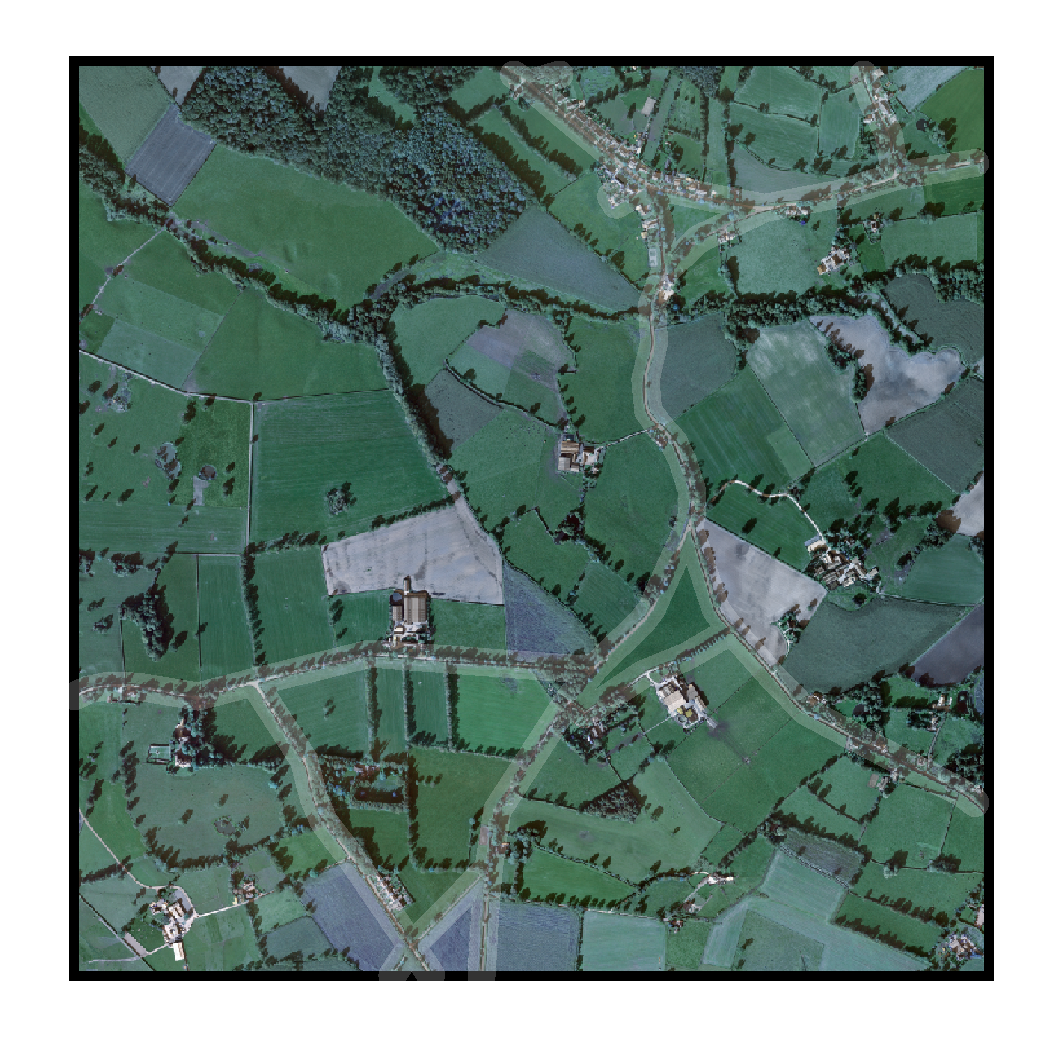
\includegraphics[width=\linewidth]{figure/area_map-1} 

}

\caption[Study area highlighting road geometries outlined in a lighter 30m buffer]{Study area highlighting road geometries outlined in a lighter 30m buffer}\label{fig:area_map}
\end{figure}


\end{knitrout}

\section{Objective of this paper}

This paper will present a method for rural road extraction for a region in the North West of England. The methodology is produced in order to ensure scalability and automation, allowing for replication for any area where data is available. Data used will include road centreline geometries, LiDAR point cloud, and aerial imagery to extract road widths through linear probability models. Additionally, this paper aims to extract other features of roads such as elevation changes, surface quality, and the sharpness of bends. These key features aim to provide information that may inform the selection of appropriate speed limits on rural roads, where the 60mph national speed limit is inappropriate.

Key Aims:

\begin{itemize}
    \item Produce and assess an automated method using LiDAR, aerial imagery and OS road geometry to determine the true width of roads within the chosen study area.

    \item Using OS Road and LiDAR Data produce an automated method for determining the characteristic of roads that relate to overall road quality.

    \item Assess the potential for speed reduction on rural roads, with the assumption that at present the roads chosen are 60mph.
\end{itemize}

The site selected in this study was chosen to include a selection of A, B, and Unclassified local roads within a rural setting. Particularly the roads chosen are often partially obscured by tree canopies and do not have visible kerbs, both key features in rural British roads.

This paper is organised into chapters, first a literature review, outlining the broad implications of speed limits, rural road networks, and object extraction particuarly in relation to LiDAR aerial point clouds. Second, a detailed description of the methodology involved in this paper will outline the techniques used to classify road widths, in addition to the other road geometric information. A results section will primarily assess the method for road extraction, through sensitivity analysis and some qualitative observations, a short section will then explore the findings. Finally a discussion will detail the implications for the findings, and suggest areas for improvement.

// improve this, why am i doing this, e.g. production of method will aid speed limits, emergency response etc.

// Include more infrastructure to support the over-arching narrative argument. E.g. The intro. should include a brief overview of the argument (sections) to come [signposting], and there should be more linking sentences between sections to help the reader understand both that the focus is being changed and why.

\end{multicols}

\chapter{Literature Review}
\label{ch:literature}

\begin{multicols}{2}

    \lettrine{T}{ypical} road extraction techniques have focused purely on urban road networks and involved methods which can be both computationally intensive and time consuming. Given the pressure for full quantitative assessments of the current speed limits in the rural network in the United Kingdom, there is a demand to produce comprehensive methods for rural road feature extraction. This paper primarily focuses on techniques for assessing the road geometry for roads considered to be rural connecting roads in the United Kingdom. This literature review will first outline the current understanding of the rural road network, considering the role of speed and speed limits in accident likelihood, rural accessibility, and a detailed look at current road extraction techniques involving aerial imagery and LiDAR, presenting the key differences and limitations of these studies when considering the rural road network in the UK.

\section{British Rural Road Network}

\cite{taylor2002} conducted a comprehensive study outlining the key features of British rural roads, in an effort to improve the characterstics associated with accident rates, above that which was explored by the MASTER study which primarily consisted of European road data, with limited data for England \citep{baruya1998}. \cite{taylor2002} identify key features of 174 selected rural british roads across England which they use to classify roads into certain categories, this data was obtained through drive through video recordings.

\begin{table}[H]
\fontsize{8}{10}\selectfont
\begin{tabular}{ll}
\toprule
\textbf{Type of data} & \textbf{Examples} \\
\midrule
Discrete data & \begin{tabular}[c]{@{}l@{}}Type of junction \\ Minor junctions \\ Accesses \\ Number of bends, classified into:\\ \quad Sharp (warning signposts) \\ \quad Medium \\ \quad Slight\end{tabular} \\ \\
Semi-continuous data & \begin{tabular}[c]{@{}l@{}}Lighting \\ Reflecting road studs \\ Kerbs \\ Number of lanes \\ Road markings \\ Land use\end{tabular} \\ \\
Continuous data & \begin{tabular}[c]{@{}l@{}}Visibility \\ Verge width and type \\ Roadside type \end{tabular}                                                                                                                              \\ \bottomrule
\end{tabular}
\end{table}

Notably, the features unique to rural roads were observed to be the land use either side of a road, consisting mainly of residential, farming, wooded, open or industrial. Verges consisting of grass verges, pavement, low banks, ditches or none. Roadside type included the most dominant vertical feature closest to the road, including trees which may overhang the road, hedges, banks, fences and so on. This study also manually measured the road width for each site, and to determine the "hilliness" of roads, the number of 10m contour lines crossed were counted to give the total change in height.

\cite{taylor2002} found that the average width of British rural roads varied from 2m to 10.2m with a mean width or 6.5m. Most were two lane roads, however a small number were single track. The mean length of roads was 3km, around half the sites had more than 3 bends per km with 1 third showing 1 severe bend per km. Most roads were flat, showing less than a 10m rise per km.

Road quality in this assessment was determined through categorising roads into four key groups:

\begin{itemize}
    \item Group 1: Roads which are very hilly, with a high bend density and low traffic speed. \textit{These are low quality roads.}

    \item Group 2: Roads with a high access density, above average bend density and below average traffic speed. \textit{These are lower than average quality roads.}

    \item Group 3: Roads with a high junction density, but below average bend density and hilliness, and above average traffic speed. \textit{These are higher than average quality roads.}

    \item Group 4: Roads with a low density of bends, junctions and accesses and a high traffic speed. \textit{These are high quality roads.}
\end{itemize}

This study therefore attempted to outline a rural road hierarchy in relation to road function, and certain road geometries, which addresses issues outlined in the Government's review of speed policy \citep{departmentoftheenvironmenttransportandthe2000}. However, due to the nature of the data collection for this study, time constraints mean that producing a full road hierarchy for all rural roads within England is impractical and requires a review of the methodology. Additionally the speed policy review notes that road hierarchies should inform appropriate speeds for each road.


See \citep{taylor2000}

\subsection{Rural Speed Limits}

Accidents on rural roads often occur within the 60 mph speed limit meaning a distinction between what is an appropriate speed should be made that does not relate to a given speed limit. \cite{baruya1998} suggest a distinction between both \textit{excess} and \textit{inappropriate} speed. \textit{Excess} when driving above the speed limit, and therefore directly breaking the law, \textit{inappropriate} speed; driving too fast for the conditions of the road, not necessarily above the speed limit, often considered dangerous driving. A study by the \cite{departmentfortransport2013b} assessed the impact of inappropriate speed on rural roads, which contributed to 20\% of all crashes on minor rural roads with a 60mph limit, whereas excess speed only accounted for around 16\% of collisions. An observation of 270 single carriageway rural roads in England found that the mean distribution of speeds had a wide distribution, often significantly below the 60mph limit \citep{departmentfortransport2006}.

The Department for Transport found that rural roads account for around 66\% of all road deaths, despite accounting for around 42\% of the total distance travelled by all vehicles. Notably 51\% of all deaths in Britain in 2011 occurred on rural single carriageway roads, with the national speed limit of 60mph \citep{departmentfortransport2011}. 

\subsection{Speed, Road Geometry and Accidents}

Lowering the speed limit on roads has been shown to result in an overall reduction in the average speed of vehicles.\cite{finch1994} found that a reduction in the speed limit of a road resulted in a mean speed reduction of around one quarter of the difference, noting that drivers will often obey speed limits that they determine to be reasonable. A reduction in average speed subsequently leads to a reduction in road traffic accidents\citep{finch1994;taylor2002},\cite{taylor2000} produced the EURO model to predict accident frequencies given the proportion of drivers exceeding the speed limit and the average speed, finding that excess speed and a higher speed limit were both associated with a higher accident frequency.  Particularly, the risk of death at various speeds has been assessed in various studies,\cite{richards2009} found that at 60mph the risk of a driver dying in a head on collision between two cars is around 90\%, but with a reduction in speed, this drops to around 50\% at 48mph.

\cite{taylor2000}  demonstrated that traffic flow, link length, and the number of minor junctions all directly increased the number of accidents, while wider roads were associated with a reduction in the number of accidents. The \textit{MASTER: Speed-accident relationship on European roads} \citep{baruya1998}, assessed road geometry and other features of roads, however road data for the United Kingdom was limited to a small area in the South East, suggesting that a comprehensive methodology for the extraction of UK rural road geometry is required for a more comprehensive study.

Developed speed tool:
\citep{departmentfortransport2013a} Straightforward method for determining appropriate speed limits.Forcasting speed reduction and therefore accident reduction with revised speed limits. Does not take into account road geometry etc.

\subsection{Accessibility}

Rural accessibility can be defined in terms of economic and social opportunity as the proximity or ability for spatial interaction \citep{gutierrez2009}. In relation to transport specifically, accessibility may be defined as the ability or opportunities by which basic services can be reached by either public or private transportation \citep{gutierrez2009}.

Journey time on rural roads is often a primary concern when considering a reduction in speed limits, often higher speed is perceived to bring with it shorter travel times, and greater accessibility for people and goods \citep{departmentfortransport2013b}. Despite this, there is evidence to support that traffic travelling at constant, and lower speeds may result in overall more reliable journey times, and the time saved by travelling at faster speed is often overestimated \citep{stradling2008}.

Despite this, transport accessibility for rural communities is far more limited than for urban communities, where often rural areas have limited or no public transport, meaning there is a heavy reliance on personal transport \citep{gray2001}. Accessibility in this context can be defined as the transport facility or opportunities with which basic services can be reached from a given location by using a certain transport system \citep{gutierrez2009}.

There has been little focus on the improvement of transport technologies in rural areas, with the potential for new technologies implemented into urban areas improving rural accessibility \citep{velaga2012}. A key area to address is the level of accessibility to hospital services for rural communities, where recent centralisation of these services has negatively impacted the level of access for rural communities \citep{mungall2005}. This also impacts the level of access for hospital services to reach rural areas, where distance and time taken to a hospital directly correlates with a patients mortality \citep{nicholl2007}. Emergency vehicles are often larger than personal vehicles and as such it can be assumed that accessibility for these types of services is often more limited depending on the quality of rural roads.

\cite{velaga2012} conducted a study outlining the key transport and technological challenges that limit accessibility within rural areas, demonstrating that the quality of rural infrastructure, and access to services are key factors driving social exclusion and limited access to goods and services. \cite{velaga2012} suggest that technological innovations targeting rural areas may alleviate this problem through the production of user generated data, they note that certain challenges will come with this technology, notably their first point;

\begin{quote}
Understanding basic technological infrastructure requirements in rural areas.
\end{quote}

Suggesting a greater understanding of the existing rural road infrastructure is required before the introduction of existing rural technologies may improve access to rural areas.

More on emergency response.

// expand all, summarise the mentioned papers.

\subsection{Road Maintenance}

\citep{yadav2018}: road surface three dimensional information important for pavement condition asessment, road maintenance citep Mcelhinney2010; yang2013

\citep{jaakola2008}
information can be obtained with airborne laser scanning at low altitudes.
When the road has been constructed, documentation of road information is needed for an increasing
number of other applications, such as noise modelling, road safety, road maintenance, location-based
services, and car and pedestrian navigation. Documentation of the road environment includes
documentation of both road geometry and road environment.
Road geometry means the parameters used for the geometric design of roads, such as design speed,

\section{LiDAR Data Classification}

Aerial LiDAR classification typically follows two objectives, the classification of ground and non-ground points, and the classification of surface objects, including buildings, trees or roads \citep{charaniya2004}. Classification takes two forms, \textit{supervised} and \textit{unsupervised}, supervised classification taking a \textit{training} dataset and using it to estimate the paramaters associated with the outcome hoping to be classified. These parameters are then used on unknown data, with a similar distribution to the training set, and used to classify features \citep{charaniya2004}.

\subsection{Digital Terrain Models}
\label{subs:dtm}

Early LiDAR classification primarily focused on the production of digital terrain models (DTM), \cite{kraus1998} used an iterative linear prediction algorithm which used residuals to compute weights for each point. Ground points produced residuals with negative weigthing, and vegetation was more likely to produce residuals with higher weighting. From this 47.8\% of points were classified as vegetation, from this they note that advances in the technology, such as the inclusion of multiple laser pulses enable for a higher quality DTM.

\cite{vosselman2000}, proposed a laser pulse filtering technique for distinguising laser points that were reflected from buildings and vegetation, than those from ground, weights were assigned to points, determined by an assigned acceptible height difference between two neighrbouring points. Limitations at the time of this study meant that processing requires points to be aggregated into a grid for processing, resulting in significant information loss. Results were generally good for the simplicity of the method, giving a RMS error of 20-30cm, however \cite{vosselman2000} note that this error likely does not reflect the true precision of the DEM, which may be slightly worse.

The observation of height textures are another method for DEM extraction enabled through the use of LiDAR data. \cite{maas1999} used height variation between neighbouring LiDAR points to classify buildings, trees, and flat terrain, with enough detail to detemrine whether a building had a flat or sloped roof. Similarly\cite{elberink2000} noted that man made structures often have smooth, regular height textures, with small variations in height, while trees and other vegetation give an irregular height pattern. Empirical assessment of the accuracy of their technique resulted in a 98% accuracy for buildings, and 97% for trees, however ground based objects could only be detected with an accuracy of below 70% and\cite{elberink2000} suggest that multi-spectral data should be included to achieve better results.

\cite{zhang2003} used morphological filtering of points assigned into a regular grid by inputting a minimum elevation for each cell in the grid, and interpolating the elevation of cells not containing any points. Accuracy of the results were assessed both quantitatively and qualitatively, giving 3\% error from misclassified points, however observation of the DEM showed artefacts primarily from larger buildings.

This paper will utilise a recent method for DEM production in order to classify ground and non ground points for subsequent road classification. The method chosen was proposed by \cite{zhang2016} uses \textit{cloth simulation} to generate a DTM from LiDAR data. This algorithm, unlike other filtering algorithms, allows for a simplistic input, without the need for numerous parameters to ensure an accurate DTM. This method consists of four main steps:

\begin{itemize}
    \item \textit{Initial State} A cloth is placed above the inverted LiDAR measurements.
    \item The displacement of each LiDAR point is calculated under the influence of gravity, meaning some points appear below ground measurements.
    \item \textit{Intersection check.} For any points detected as being under the ground, they are moved to ground level and set to be unmovable.
    \item \textit{Considering internal forces.} Movable points are moved according to neighbouring points.
\end{itemize}

Quantitative accuracy of this methodology gave results similar to top existing DTM production algorithms, but with a far more simplistic implementation.

\subsection{Feature Classification}

Developments in LiDAR enabled the possibility of classification by using laser intensity information and multiple returns, features of more advanced LiDAR systems. The TopEye system used by \cite{axelsson1998} allowed for  classification of buildings and electrical power-lines using reflectance ($1/intensity$) to obtain radiometric information about the area and note that this can be used to separate paved area from grassland. Power lines in particular benefited from the multiple returns produced by the LiDAR system used as they often gave one return from the power line, and one from ground.

// if i want more,...
 Maas [12] height texture for segmentation of lidar. Filin [5] surface clustering technique for identifying regions in lidar exhibiting homogeneity in certain feature space consisting of postion, tangent plane, and relative height difference attribures for every point. the surface are categorised as hiehg vegetation, (height jumps), low vegetation, smooth surfaces and planar surfaces // note that smooth surfaces often man made (find ref). song [17] separation of materials, trees grass ashphalt, roads, and roofs on intensity data, interpolated using three trechnqies, idw, median filtering and kriging. Hebert [7] presented outling or some classification.
Approaches using mixture models [14,10,4,3] for paramatric classification. Maceda [9] ground based laster discriminting grass and rocks. 
Inclusion of aerial imagery, improvement of classification [2], or others [13,15].


Ground based lidar: \citep{yadav2018}


\section{Road Classification}

// small history of road extraction here
// list varying resolution increases per papers?
// timeline of aerial image quality/lidar
// Note that as they use point density of 1/2m, and intensity has a footprint of 20 - 30cm the intensity if not typically used. (Rottensteiner, 2003). **with my method we use a resolution of 25cm, much higher point density**

In comparison the extraction of vegetation and buildings from LiDAR, the extraction of roads poses far more of a challenge, due to there being less prominent height differences \citep{vosselman2009a}. Road classification is essentially a data clustering method to categorise data into road and non-road points, enabled through discovering patterns and relationship between variables and validation of findings \citep{saeedi2009} Clustering may be achieved through various algorithms, categorised generally into partitioning methods, hierarchical methods, density-based methods, grid-based methods, and model-based methods \citep{saeedi2009}.\cite{yadav2018} note that the periodic assessment of roads is greatly important due to the increasing traffic load, and new automated techniques will enable this in areas where in the past it had not been feasible. Due to the heterogeneous nature of certain roads types, the road environment is often complex, meaning collection and accurate processing of road features is challenging \citep{yadav2018}.


Road classification methodologies have historically used purely aerial imagery, providing only road pixels and 2D location information \citep{yadav2018}. \cite{ferchichi2005} used high resolution satellite imagery for road centreline extraction from a suburban area based on cluster coverage. They used image segmentation through maximum likelihood to assign pixels to road and non-road classes, making the assumption that both classes gave a Gaussian distribution. Features for classification include the angular second-movement, contrast, and entropy of the image, based off image texture analysis by \cite{dubes1992}. Results of the classification gave significant noise, noted as a possibility due to non conformance with a Gaussian distribution, however, centreline extraction from the resultant classification removed any pixels with low density and ran a $K$-means clustering algorithm iteratively to determine road clusters. \cite{wan2007} produced an automated method for mapping urban and suburban roads using high resolution satellite imagery, using spectral, context, shape and the structural features or roads. Using fuzzy segmentation, classification of buildings, parking areas, and road clusters were obtain, but with large levels of noise. Angular texture analysis was able to reduce this noise, however large areas of incorrectly classified roads appear present results. Additionally, while not mentioned in this study, the method proposed fails to address the differentiation between road and pavement, a key issue with the use of 2D imagery. \cite{hormese2016}: automated road extraction from high res satellite images. new availability of v high res sattelite,( not aerial )


\subsection{LiDAR Road Classification}

The majority of current road classification techniques using LiDAR have focused on unsupervised classification, often with the goal in vehicle automation using mobile LiDAR data \citep[][e.g.]{yadav2018;kumar2013;smadja2010;jaakola2008}. Applications using aerial LiDAR have also followed this trend for unsupervised classification. \cite{clode2004} used a sequential Hough filtering transformation to classify roads using aerial LiDAR data, achieved by first taking only the last pulse LiDAR coordinates, considered a digital surface model (DSM)\footnote{Contaning all surface objects, including ground points, vegetation, and man made structures such as buildings and roads.}. To obtain a DTM from the DSM, \cite{clode2004} used a method as proposed in \cite{rottensteiner2003}, using a square structural element and grey scale opening to filter non-terrain objects. \cite{clode2004} note that at the time of production, intensity data with LiDAR had been often subject to large amounts of noise, and their use of intensity values for road detection was only a recent possibility. Road classification was subsequently achieved through both intensity and height filtering. Minimum and maximum intensity values for the road surface type (bitumen) were used to remove points that fell outside these values, and points that were outside a selected tolerance from the DTM were also removed. This methodology achieved a completeness of 86\%, correctness of 69\% and quality of 65\%, quantified by the use of a ground truth model. This methodology provides a simplistic method for unsupervised road classification that reached similar levels of accuracy as more complex methods for the time, at the expense of certain assumptions, namely the road surface material.

Many methods for road classification from LiDAR follow similar patterns, first identification of ground points through height data, and DTM extraction through interpolation, and subsequent classification based on the attributes of the point cloud \cite{vosselman2009}. Due to the 3D information provided by LiDAR data, kerbs can be segmented from roads, achieving a more accurate road edge location when kerbs are present. However, due to the often small jump between kerb and road, this methodology is limited to new terrestrial mobile LiDAR data collection.\cite{jaakola2008} produced a methodology using mobile LiDAR data to classify road edges by segmenting kerbstones based on the height gradient along the scanned profile, with a final completeness of 73.9\%, and correctness of 85.6\%. Additionally, road markings were segmented from the road surface using intensity information. The mobile data collection for this study obtained a point resolution of between 10cm$^2$ and 100cm$^2$, with driving speeds of 20km/h to 50km/h. \cite{jaakkola2008} note that due to the size of the data produced through this method, computation times were lengthy. \cite{yoon2009} similarly developed an approach for urban drivable terrain detection for automated vehicles through mobile LiDAR data, road edges were obtained through the slope and standard deviation of the height of points, finding the standard deviation to be far more efficient for edge detection. They note that while results were promising, it would take a very long time to collect data for a large number of roads, and at higher vehicle speeds, LiDAR points density is reduced below a usable threshold. 

//- Extraction includes detection of planar or smooth surfaces, and the classification of points or point clusters based on local point patterns, echo intensity and echo count information \citep{vosselman2004;darmawati2008}

// elberink2009: automated method for 3d modelling highway infrastructure using airborne LiDAR + 2d topographic. Road polygons were extracted from the topographic map data using a map based seed-growing algorithm combined with a Hough transformation. points added to the correspondng road polygons using a LiDAR based seed-growing algorithm then mapped polygons

// 2. Lidar points distirbute irregularly with non uniformity density. the point density in the overlapping area between fight strips is greater than non-overlapping regions. There is no point in areas occulded by tall objects. can be soled interpolating into intensity image (e.g. Zhao,2012, zhu 2009) binary image, Clode 2007. others see Samadzadegan 2009, Jiangui 2011.

// Vosselman2009, developed a method for detecting kerbstones from airborne LiDAR data, based on the detection of small height jumps caused byt he kerbstones in the LiDAR point cloud data. Cars parked occluded kerbstones. \cite{vosselman2009a} used low flying airborne LiDAR point cloud data with a very high density of 10-20m$^2$

\subsection{Supervised Methods}

// Few supervised methods for road classification exist summarise these: \cite{guan2013;hul2008;dahlkamp2006;matkan2014;ferraz2016;charaniya2004}. 
//  ALSO SUPERVISED: - Hatger and Brenner 2003,2005, laser scanning data at 0.5m to extract properties of roads for which centrelines arer known from a road database. Including height longitudinal and transversal slope, curvature, and width. Height profiles across road split into straight sgements. A RANSAC procedure on the end points of the sements with low slope values is used to fit straight lines to the road sides. \citep{hatger2003;hatger2005}

Charainya gives information which is utilised in this paper for the modelling. i.e. Lum and Intensity are most useful for road detection

// summary:


\subsection{Rural Road Extraction}

See \citep{kumar2013}:
Majority attempt to delineate roads by distinguishing them from non-road objects but do not attempt to extract the road edges. Most for urban roads, rely on sufficient height or slope difference between the road and kerb points for etecting road sedges. Little or no research been carried out to extract rural roads, wheer non-road surface comprises grass-soil and edges not as easily defined by slope changes alone. Intensity and pulse width attributes from liDAR data can be a useful source of intermation for extracting these roads edges. 

\citep{yadav2018}: Major limitation of existing methods to extract rural road surface as mostly without curb. Methologies such as Yang et al., 2013 which deals with curbs and boundaries characterized as ashpalt/soil and ashpalt vegetation and ashpalt/grassy bank. Exact edge location difficult if point density less and sufficiant elevatio jump not present at boundary of carriageway (Mc Elhinney et al., 2010). Wu et al., 2013 dependent on road range which cannot be calculated correctly if height diffrernce between road surface and shoulder not obvious.

Key factors in determining poor road quality:
\begin{itemize}
    \item Width \citep{taylor2002} \citep{aarts2006}
    \item Surface quality
    \item Blind corners/winding roads \citep{aarts2006} \citep{wu2013}
    \item Junction Sharpness \citep{aarts2006}
\end{itemize}

// read these papers and identify why these should be considered when assessing road quality

\end{multicols}

\chapter{Methodology}
\label{ch:methods}

\begin{multicols}{2}
    This paper primarily makes use of the free open source statistical language \R{} \citep{rcoreteam2019}. Managing the large LiDAR datasets from my personal computer was mode possible through the \texttt{lidR} \R{} package \citep{roussel2019}. Further details regarding the \R{} environment and computer setup used for this paper is given in \textbf{Appendix \ref{a:code}}. All content was written using \LaTeX{} combined with the \texttt{.rnoweb} file type \citep{ihaka2011}, for \textit{Literate Programming}\footnote{See \cite{knuth1984}}. The template is built from scratch but takes much inspiration (and code) from the \href{https://github.com/asardaes/R-LaTeX-Template}{R-LaTeX-Template}.

    All code is hosted on my personal \href{https://github.com/cjber/}{GitHub account}. Also hosted are my complete dotfiles, used in conjunction with the Linux distribution Manjaro, with the i3 window manager. All writing and code was produced using \href{https://neovim.io}{\texttt{neovim}} with my personal configuration to implement integrated development environment (IDE) style features for writing R code, while also providing essential features for writing in \LaTeX{}. \texttt{neovim} has the benefit of being both highly customisable, and lightweight, which allows for much lower system utilisation compared with R Studio when working with large datasets. One essential \texttt{vim} package to mention is the \href{https://github.com/jalvesaq/Nvim-R}{Nvim-R} vim package.

    Given in Appendix \ref{a:code} are the code snippets utilised in this methodology, for many equations, the relevent code is given as a reference to the appendix location.

\section{Data}
\label{sec:data}



LiDAR point cloud data was downloaded through the \href{https://data.gov.uk/}{UK Government's open data repository} which uses the \href{http://www.nationalarchives.gov.uk/doc/open-government-licence/version/3/}{Open Government Licence}, allowing for:
    \begin{itemize}
        \item Copying, publishing, distributing and transmission of the data
        \item Adaptation of the data
        \item Commercial and Non-commercial use of the information
    \end{itemize}

    LiDAR data used in this paper is available \href{https://data.gov.uk/dataset/977a4ca4-1759-4f26-baa7-b566bd7ca7bf/lidar-point-cloud}{\textsc{here}} under this licence \citep{ukgovernment2019}. This data was given as a compressed LAS file format (\texttt{.laz}), the \R{} package \texttt{lidR} provided the function \texttt{catalog()} which enabled each separate \texttt{.laz} to be combined into one object of class \texttt{LAScatalog}. Analysis on this object could then be split into chunks (selected as 500m$^2$), allowing for multi-core threading to speed up analysis, and a reduction in the memory overhead when reading in data, often a limitation of the \R{} language as objects are stored entirely into memory when read \citep{wickham2014}. The \texttt{LAScatalog} object did not require the compressed \texttt{.laz} files to be read into memory as \texttt{.las} files, meaning memory limitations were far less of a problem.

    Aerial imagery was downloaded through \href{https://digimap.edina.ac.uk/}{Digimap\textsuperscript{\textregistered}
    } which uses the \textit{Aerial Digimap Educational User Licence}, allowing for free use of the data for educational purposes \citep{theuniversityofedinborough2019}.

Road centreline geometries were accessed through the \href{https://www.ordnancesurvey.co.uk/business-and-government/products/opendata.html}{Ordnance Survey Open Data repository} which shares the Open Government licence. These were downloaded in the GeoPackage format (\texttt{.gpkg}) nationally and cropped to the extent of the LiDAR point cloud data.

\section{LiDAR Preprocessing}

The total number of LiDAR points used in this study is 9,419,272. All LIDAR data has a vertical accuracy of +/-15cm Root mean square error (RMSE). An overview of the LiDAR data selected for this study is given on Table \ref{tab:lidartab}. The variables of primary interest are:

\begin{itemize}
    \item \textbf{Z:} The distance a laser pulse is reflected back to to scanner, calculated by the time taken for a return pulse to be detected.
    \item \textbf{Intensity:} The amplitude of the return pulse, reflected back by the surface terrain or objects.
	\item \textbf{ReturnNumber:} A number of range 1-5, indicating for a point, the corresponding order of a reflected laser pulse. A ReturnNumber of 1 indicates the first return for a pulse (and highest $z$ value), a return number of 5 indicates the last return (and lowest $z$ value).
	\item \textbf{NumberOfReturns:} The number of return pulses for a single laser pulse (maximum of 5).
    \item \textbf{Classification:} A number given to a point indicating a specific numeric classification. Of interest in this study is a classification of 2, indicating a ground point. More information can be found \href{http://desktop.arcgis.com/en/arcmap/10.3/manage-data/las-dataset/lidar-point-classification.htm}{here}, which outlines numerical classifications for various vegetation types and man made structures.
\end{itemize}



\begin{table}[H]

\caption{\label{tab:lidartab}LiDAR Point Cloud Summary Data}
\centering
\fontsize{8}{10}\selectfont
\begin{tabular}{lrrrr}
\toprule
\textbf{ } & \textbf{Mean} & \textbf{SD} & \textbf{Min} & \textbf{Max}\\
\midrule
Z & 80.55 & 5.95 & 64.85 & 115.79\\
Intensity & 176.57 & 125.08 & 1.00 & 4064.00\\
ReturnNumber & 1.47 & 0.95 & 1.00 & 5.00\\
NumberOfReturns & 1.95 & 1.42 & 1.00 & 5.00\\
ScanDirectionFlag & 0.50 & 0.50 & 0.00 & 1.00\\
EdgeOfFlightline & 0.00 & 0.03 & 0.00 & 1.00\\
Classification & 3.04 & 1.70 & 1.00 & 8.00\\
ScanAngleRank & -1.97 & 13.18 & -22.00 & 22.00\\
\bottomrule
\end{tabular}
\end{table}





\subsection{Last Pulse}

The LiDAR point cloud data used in this paper gives the values for 5 pulse returns. The canopy above roads may be excluded through ignoring early pulses (higher Z values), therefore only the last pulse values for any point are selected, this can be expressed as;

$$
\mathbf{p}_{i}=(l p x, l p y, l p z, l p i),
$$
\begin{flushright}
    \footnotesize{\ref{code:lidr_clean}}
\end{flushright}

where $\mathbf{p_i}$ is a single instance of a LiDAR point within the chosen point cloud, $lpx$ is the last pulse $x$ coordinate, $lpy$ the last pulse $y$ coordinate, $lpz$ the last pulse $z$ coordinate, and $lpi$ the last pulse intensity value.

\subsection{Normalisation}

Ground points were classified using the Cloth Simulation Filtering (CSF) algorithm, as described in \cite{zhang2016}. Points were already classified in the data provided, however, as the classification technique was unknown, reclassification was considered necessary. The general implementation simulates the movements of a piece of cloth lying over the inverse of a point cloud, as the point cloud is flipped, the cloth settles beneath ground points, while covering points that lie separate to the ground, essentially forming a digital terrain model (DTM), cloth simulations are described in more detail in \cite{bridson2005} and subsection \ref{subs:dtm}. The CSF algorithm is given;

$$
X(t+\Delta t)=2 X(t)-X(t-\Delta t)+\frac{G}{m} \Delta t^{2},
$$
\begin{flushright}
    \footnotesize{\ref{code:lidr_clean}}
\end{flushright}

where $m$  is the mass of a single LiDAR point (set to 1), $\Delta t$ is the time step between points and $G$ represents the gravity constant.

With the classification of ground points, (given $Classification = 2$), a full DTM may be produced through spatial interpolation of the classified points. This process is called normalisation, and ensures that when extracting height information, any observed values are due to objects on the surface of the terrain, and not due to the lie of the terrain itself. Interpolation uses the inverse distance weighting and $k$ nearest neighbours algorithms to produce the DTM. Nearest neighbours were selected as $k = 10$, with $p = 2$ for the inverse weighting, and used to produce a DTM with a resolution of 1m. This particular technique was selected over more comprehensive methods such as kriging as the number of points is very high, and the small benefit was considered minimal compared with the increase in computational load. The $z$ values from the DTM were then subtracted from the LiDAR point cloud, leaving a normalised point cloud.

\subsection{Points Extent}

With the normalised last pulse point cloud, the point cloud was clipped to within a 30m extent of each known road location, using the OS road shapefiles. Selecting a 30m extent ensured that even with slight inaccuracy in road location, the road LiDAR points would likely not be excluded. A large number of unimportant points were therefore removed, saving on computational resources. Additionally this extent ensured that both road and non road points were included, but reduced the chance of false positives from occuring as fewer non road points were now included in the analysis.

\section{Road Analysis}
\label{sec:road-extraction}

This section combines data extracted through the OS road shapefiles preprocessed LiDAR data, and aerial imagery to obtain a set of creteria to assess the chosen road network. These criteria are;

\begin{itemize}
\itemsep0em
    \item Road Width
    \item Bend Sharpness
    \item Road Steepness
    \item Surface Quality
\end{itemize}




\begin{table}[H]

\caption{\label{tab:roadstab}OS Roads Data Summary}
\centering
\fontsize{8}{10}\selectfont
\begin{tabular}{l>{\raggedright\arraybackslash}p{12em}}
\toprule
\textbf{ } & \textbf{Example}\\
\midrule
id & idE381337E-E88D-4232-8CAD-F543F178EBE4\\
endNode & id42B6F387-D838-445C-AA7A-6558362B7B9F\\
startNode & idC8EE8B4C-D965-436A-BA02-A0925A6EA1B8\\
roadNumberTOID & osgb4000000013398492\\
roadNameTOID & \\
fictitious & FALSE\\
roadClassification & B Road\\
roadFunction & B Road\\
formOfWay & Single Carriageway\\
length & 241\\
loop & FALSE\\
primaryRoute & FALSE\\
trunkRoad & FALSE\\
roadClassificationNumber & B5392\\
name1 & \\
name2 & \\
roadStructure & \\
\bottomrule
\end{tabular}
\end{table}



\subsection{Road Sampling}

The LiDAR point cloud data was sampled at regular 10 meter intervals for each road, perpendicular to the road direction, ensuring that when road directin changed, the sampling locations remained perpendicular. Each road was first split into nodes at which road direction changes, and from this, points at 10 meter intervals between two connected nodes were calculated;
$$
p_k = p_1 + |p_2 - p_1| \times I_k
$$

where $I_k$ is the interval value which increases by 10 meters until the length of the total distance of the node, given $I_{1}, I_{2}, \dots, I_{k}>0 and k \geq 2$.

\[
\begin{aligned}
    I_k &= (L_k + 20) - T_k \\
    L_1 &= 20 \\
    T_k &= T_{k-1}  + E
\end{aligned}
\]

where $L_k$ is the distance from the start of the node to the current sample line position, $T_k$ is total length of all nodes within a road from the start of the road and $E$ is the euclidean distance between two nodes.

To calculate the sample locations, perpendicular to the roads, first the $x$ and $y$ euclidean distances from a reference point $p_k$ and the end of the current node $n_2$ were calculated;

\[
\begin{aligned}
    len &= \sqrt{(n_{k+1} - p_k)} \\
    len_n &= (n / len) \times (n_{k+1} - p_k)
\end{aligned}
\]
\begin{flushright}
    \footnotesize{\ref{code:perp}}
\end{flushright}

from this, the lengths were inverted, giving two points of distance $n$ from $p_k$. Inversion was achieved by subtracting the given $len_n$ $x$ value from $p_k$, while adding the $len_n$ $y$ value, and vice versa. These perpendicular sample lines were buffered to a width of 1m, giving a total area of 20m$^2$ per sample and spatially joined to the existing LiDAR point cloud data, removing any points that fell outside the sample lines.

\begin{flushright}
    \footnotesize{\ref{code:compute_samples}}
\end{flushright}

\section{Aerial Imagery}

With the perpendicular sample lines extracted for the length of every road, to assist with the prediction of correct road locations, true colour aerial imagery was included. This imagery was first converted from three band RGB raster images, to a single-band grey-scale raster brick with values ranging 0 to 255, considered to be luminescence information.

$$
    luminescence = (Band_1 + Band_2 + Band_3) \div 3
$$
\begin{flushright}
    \footnotesize{\ref{code:lm_compute}}
\end{flushright}

To exclude as much noise as possible from both the LiDAR point cloud intensity information, and aerial luminescence, only points with the ground classification ($Classification = 2$), and points with only a single laser return pulse were included in the models ($NumberOfReturns = 1$).

\subsection{Linear Probability Model}

Individual linear probability models were constructed for each sample location for each road, giving results for a cluster of points across a perpendicular segment of each road every 20m. Road centrelines were selected as the outcome variable, provided by the OS road network line shapefiles, buffered to 1m to ensure a three dimensional cross section of points. Additionally, global linear probability models were constructed, and compared against the individual linear models.

Models were constructed using a maximal approach, selecting all appropriate predictor variables, iterating through models by removing variables that did not significantly influence the model outcome, or created noise.

An additional variable $Dist$ was included, representing the shortest distance from a point to the centreline of the road it is associated with, considering that road points should be weighted more towards points that are closer to the centre-point of the road.

Predictions for each point were then ran using each model, which gave the likelihood a point was either road or non road. As the likelihood values from the predictions gave a range of numerical values, points that fell below a certain threshold were removed, leaving only points that were most likely correctly identified as road points. This threshold was selected as the $95\%$ quantile for each sample point;

\[
\begin{aligned}
\mathbf{S} &= \Big(\mathbf{p}_i \in \Big[\frac{95}{100} \times \mathbf{p}_{i_{lpi}}\Big]\Big) \\
\end{aligned}
\]

Where $\mathbf{S}$ is the total point cloud.

Some points considered to be noise were still present, but often isolated. To ensure no isolated points were present, the time interval between two neighbouring points was checked, if a large time interval was found, the isolated point was removed.

$\mathbf{S}_i$ now consisted of a collection of predicted road points for each sample line along a road segment, excluding sample lines partially or fully obscured by tree canopy. To obtain road widths from these points, the maximum distance between two points in a particular sample was determined, these points were kept and all others removed. A linear section of road with two samples resembles \ref{fig:sample_points};

\begin{center}
\begin{tikzpicture}[scale=2]

\draw[-, very thick, color = gray] (0,0.5) -- (0,4);

\filldraw (-1,1) circle[radius=1pt] node [below left] {$A_1$};
\draw[-] (-1,1) -- (1,2);
\draw[dashed] (-1,1) -- node[fill=white,inner ysep=3pt, inner xsep = 3pt]{$O_A$} (1,1) ;
\draw[dotted] (1,1) -- (1,2);
\filldraw (1,2) circle[radius=1pt] node [above right] {$A_2$};

\draw(.85,1)--(.85,1.15)--(1,1.15); % right angle

\draw[<-] (-.6,1) arc (0:55:.2);
\node[] at (-.5,1.12)  {$\theta_A$};

\filldraw (-1,4) circle[radius=1pt] node [below left] {$B_1$};
\draw[-] (-1,4) -- (1,3);
\draw[dashed] (-1,3) -- node[fill=white,inner ysep=3pt, inner xsep = 3pt]{$O_B$} (1,3);
\draw[dotted] (-1,3) -- (-1,4);
\filldraw (1,3) circle[radius=1pt] node [above right] {$B_2$};

\draw(-.85,3)--(-.85,3.15)--(-1,3.15); % right angle

\draw[->] (.6,3.2) arc (135:200:.2);
\node[] at (.4,3.12)  {$\theta_B$};

\end{tikzpicture}
\end{center}
\captionof{figure}{Road LiDAR points at maximum distance apart for each sample location. Showing two example sample locations ($A$ and $B$), road centreline represented by the thick grey line. True road width is indicated by the dashed lines $O_A$ and $O_B$.}



To determine the width of the road section, according to the final two selected points at every node, pythagoras could be used to find the opposite line length, perpendicular to the road segement, considering the distance between the two points to be the hypoenuse of a right angled triangle (\ref{fig:sample_points}). The averge width for each road identifier was then found.

$|K_1K_2| = Hypotenuse$, $O_K = Opposite$, therefore $O_K = |K_1K_2| \times cos(\theta_K)$

\section{Road Angles}

The angle of bends in roads were identified through the nodes produced in the creation of the road shapefiles. First the road linestrings were split into points, with coordinates representing each node within a road, a point at which the orientation of the linestring is altered.

The bend in a road was considered to be the \textit{bearing angle} $\theta$, from a point $A\left(a_{x}, a_{y}\right)$ to a point $B\left(b_{x}, b_{y}\right)$, with the angle measured in a clockwise direction from north. This can be represented as a figure;

\begin{center}
\begin{tikzpicture}[scale=7]

\filldraw (.2,.4) circle[radius=.3pt] node [below left] {$A$};

\draw[-] (0.1,.4) -- (0.3, .4);
\draw[-] (0.2,.3) -- (0.2, .5) node[above] {$N$};

\filldraw (.8,.7) circle[radius=.3pt] node [above right] {$B$};

\draw[-] (0.2,.4) -- (0.8, .7);

    \draw[<-] (0.28,.44) arc (45:90:.111);
    \node[] at (.25,.5)  {$\theta$};
\end{tikzpicture}
\end{center}
\captionof{figure}{Bearing Angle Between Road Segments}

To find the angle $\theta$, the point $B$ can be represented into relation to point $A$ as;

$$
\left(b_{1}, b_{2}\right)=\left(a_{1}+r \sin \theta, a_{2}+r \cos \theta\right)
$$

Where $r$ is the length of the line segment $AB$. Rearranging the equation for $\theta$ gives;

$$
    \tan \theta=\frac{b_{1}-a_{1}}{b_{2}-a_{2}}
$$

This equation can be rewritten to calculate the value of $\theta$ using the $\mathit{atan2}$ function;

$$
\hat{\theta}=\mathrm{atan} 2\left(b_{1}-a_{1}, b_{2}-a_{2}\right) \in(-\pi, \pi]
$$


Finally the bearing angle $\theta \in[0,2 \pi)$ is given as;

\[
    \begin{aligned}
\theta=\left\{\begin{array}{ll}{\hat{\theta},} & {\hat{\theta} \geq 0} \\
{2 \pi+\hat{\theta},} & {\hat{\theta}<0}\end{array}\right.
\end{aligned}
\]
\begin{flushright}
    \footnotesize{\ref{code:angles}}
\end{flushright}

With the bearing angle of the first line segment $AB$ for a particular road, the change in orientation of the second road segment $BC$ may be given as $\theta_{2} = \theta_{BC} - \theta_{AB}$, with additional nodes following the pattern $\theta_{k} = \theta_{N(N+1)} - \theta_{(N-1)N}$.

\begin{center}
\begin{tikzpicture}[scale=7]

\filldraw (.2,.4) circle[radius=.3pt] node [below left] {$A$};

\draw[-] (0.1,.4) -- (0.3, .4);
\draw[-] (0.2,.3) -- (0.2, .5) node[above] {$N$};

\filldraw (.8,.7) circle[radius=.3pt] node [above left] {$B$};
\filldraw (.9,1) circle[radius=.3pt] node [above right] {$C$};

\draw[-] (0.2,.4) -- (0.8, .7);
\draw[-] (0.8,.7) -- (.9, 1);

    \draw[<-] (0.28,.44) arc (45:90:.111);
    \node[] at (.25,.5)  {$\theta_{1}$};

\draw[dotted] (0.8,.7) -- (1, .8);

    \draw[<-] (0.9,.75) arc (45:90:.1);
    \node[] at (.88,.8)  {$\theta_{2}$};
\end{tikzpicture}
\end{center}
\captionof{figure}{Bearing Angle Between two Road Segments}

For each road the maximum bearing angle between two nodes was selected, as well as the average bearing angle for a certain road.

\subsection{Road Node Elevation Change}

The elevation change between two road node points was calculated by first selecting non-normalised LiDAR points at a geometric node within a 1m$^2$ area. Nodes were obtained from the OS road data, as point coordinates obtained when the linestrings were split into points. LiDAR points were then filtered by those only classified as ground, and with only a single return, to reduce the likelihood of inaccurate $z$ values from canopy or other vegetation and vehicles. The mean $z$ value of points were found for each node, and elevation change between each node was calculated. For each road the maximum elevation change was calculated, alongside the mean elevation change.

\subsection{Surface Quality}

Surface quality was assessed roughly through the range in intensity values found in each known road point, and the average number of returns for a road for sample lines not obtructed by canopy, indicated by single returns.

\subsection{Estimate of True Widths}

QGIS used to measure roughly the width at various points along each road using 25cm resolution aerial imagery.

\end{multicols}

\chapter{Results}
\label{ch:results}

\begin{multicols}{2}

\section{Overview of Data}

\subsection{LiDAR Point Cloud}

Table \ref{tab:lidartab} indicates that there are likely some points with noise, particularly reflected by the highest intensity value (4063) relative to the mean value (187). Noise exclusion techniques are described in \cite{fang2004}, this paper takes a simplistic noise filtering technique that aims to solely remove extreme outliers from the observed intensity values in the chosen data.

\subsection{OS Road Geometry}

Class differences, all singlecarriageway roads, therefore likely 60mph. Removed private roads. A roads + B roads + unclassified. Many unnamed roads, only identification possible through \texttt{identifier}, which splits roads by junctions.

Histograms?

\section{Data Preperation}

Covers script 00.



from \ref{fig:fig_buff} \textbf{(b)} intensities values for ground points below the tree are much lower than those that are not below trees, essentially if including returns with higher than 1 return the intensity values are more unreliable.

// find Average intensity values for first and last returns, i.e. show the shadow below trees


\begin{knitrout}\footnotesize
\definecolor{shadecolor}{rgb}{0.969, 0.969, 0.969}\color{fgcolor}\begin{figure}[H]

{\centering 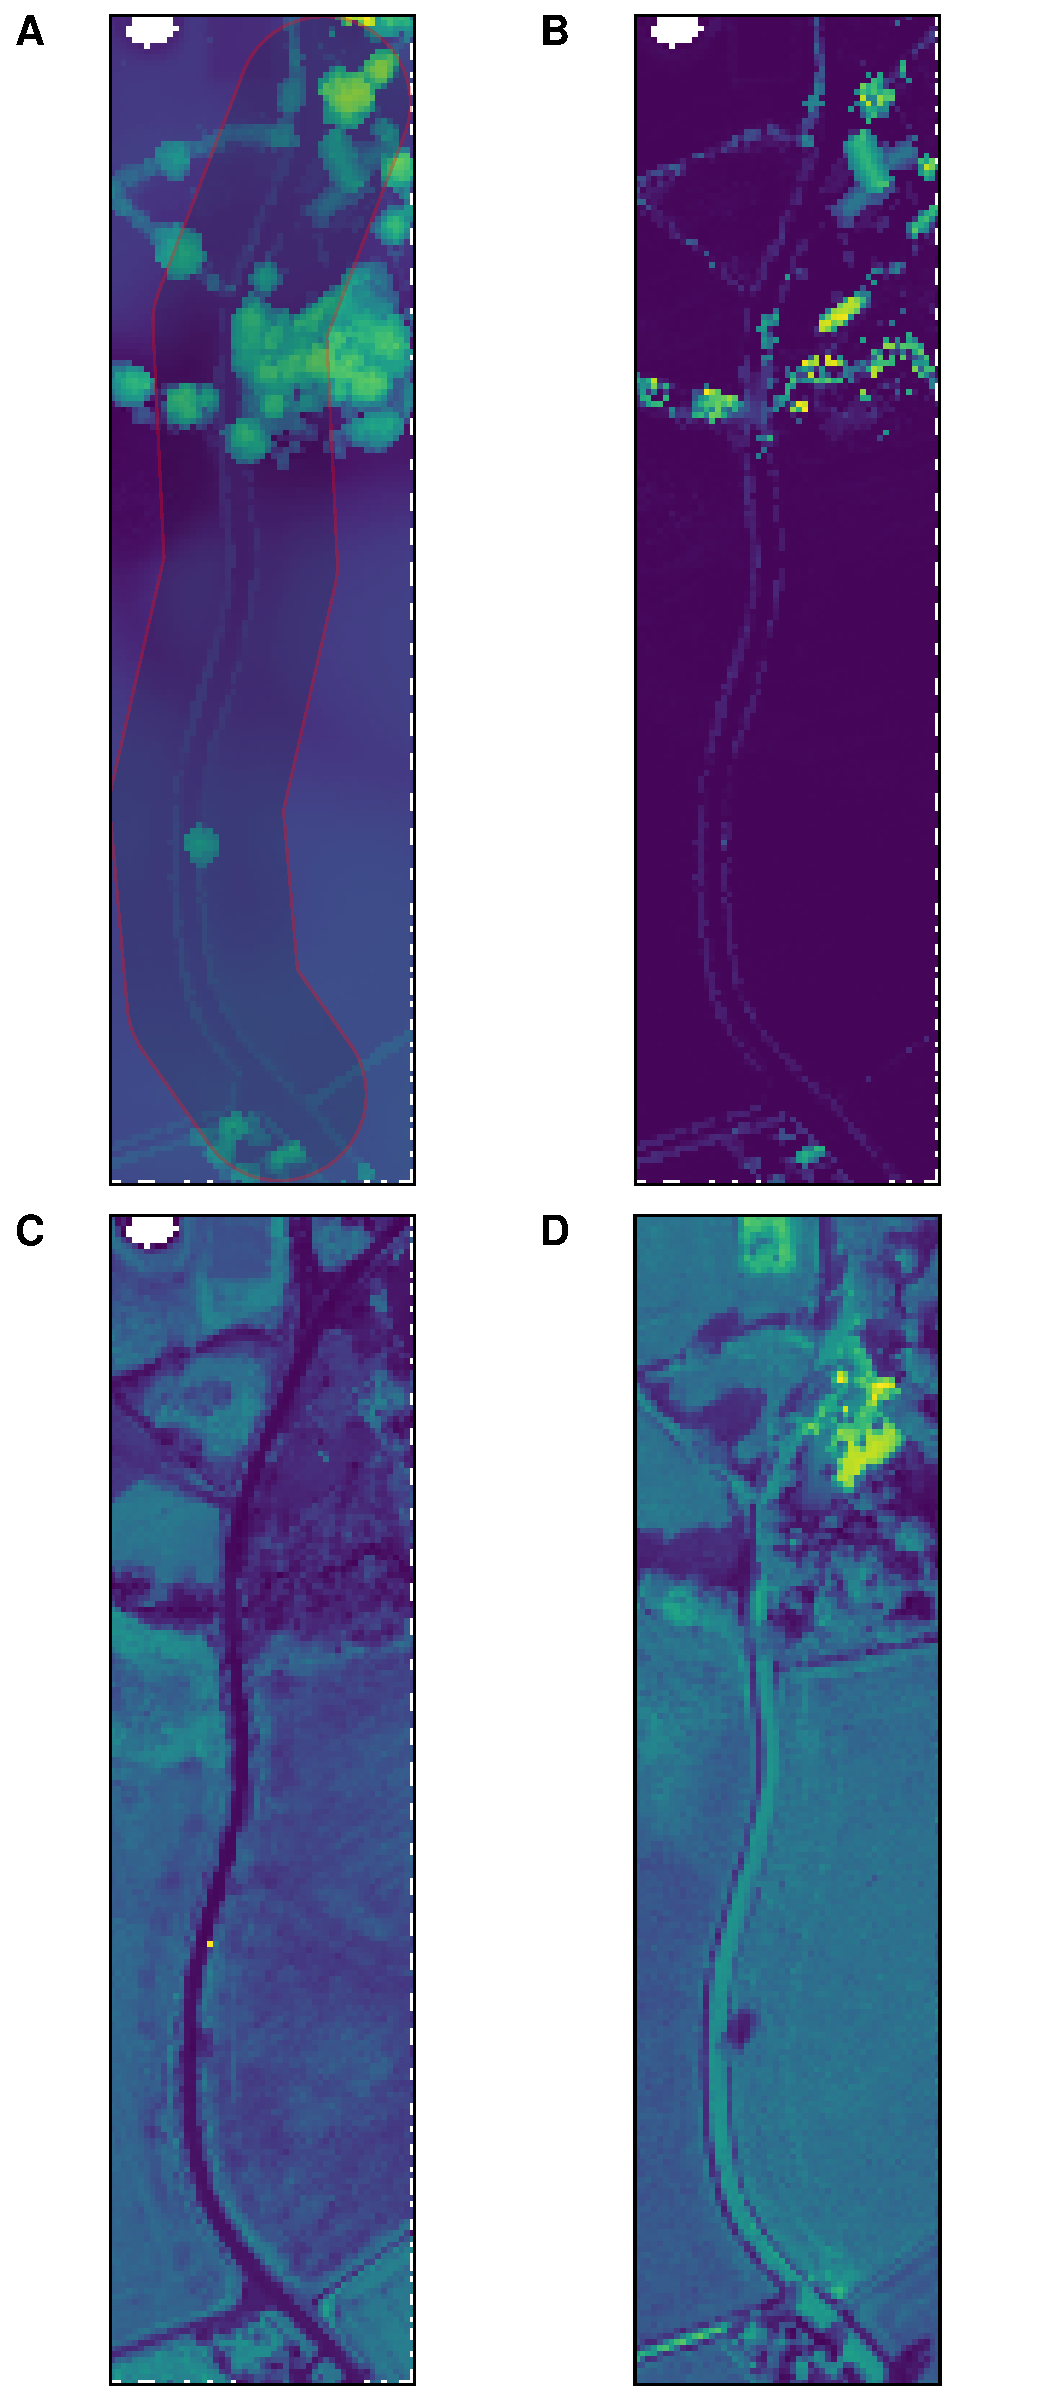
\includegraphics[width=\linewidth]{figure/fig_lp-1} 

}

\caption[LiDAR point clouds for one selected road section aggregated into 1m$^2$ grids, \textbf{(A)} Base point cloud $Z$ values, \textbf{(B)} Normalised Point cloud $Z$ values for only last returns ($lpz$) \textbf{(C)} Normalised Point cloud $Intensity$ values for last return, \textbf{(D)} Aerial Data combined to 1 band]{LiDAR point clouds for one selected road section aggregated into 1m$^2$ grids, \textbf{(A)} Base point cloud $Z$ values, \textbf{(B)} Normalised Point cloud $Z$ values for only last returns ($lpz$) \textbf{(C)} Normalised Point cloud $Intensity$ values for last return, \textbf{(D)} Aerial Data combined to 1 band}\label{fig:fig_lp}
\end{figure}


\end{knitrout}

\section{Perpendicular Sampling}

Covers 01

Show figure of sample lines. Show the reduction in number of points (memory saving)

\section{Linear Probability Model}

Covers 02


test.

\begin{knitrout}\footnotesize
\definecolor{shadecolor}{rgb}{0.969, 0.969, 0.969}\color{fgcolor}\begin{kframe}
\begin{verbatim}
[1] 0.9529064
[1] 0.9514512
[1] 0.9589439
[1] 0.9591193
[1] 0.9580487
\end{verbatim}
\end{kframe}
\end{knitrout}


First model (maximal):

//NOTES//
1. Unfiltered vs filtered global maximal model.. Filters include no samples with multiple returns (partial canopy obstruction). excludes far toomany points

2. Compare global models 1/2/3, and generalised linear model using f1.

3. Compare global model 1 (best fit), to individual model using f1.



\begin{knitrout}\footnotesize
\definecolor{shadecolor}{rgb}{0.969, 0.969, 0.969}\color{fgcolor}

{\centering 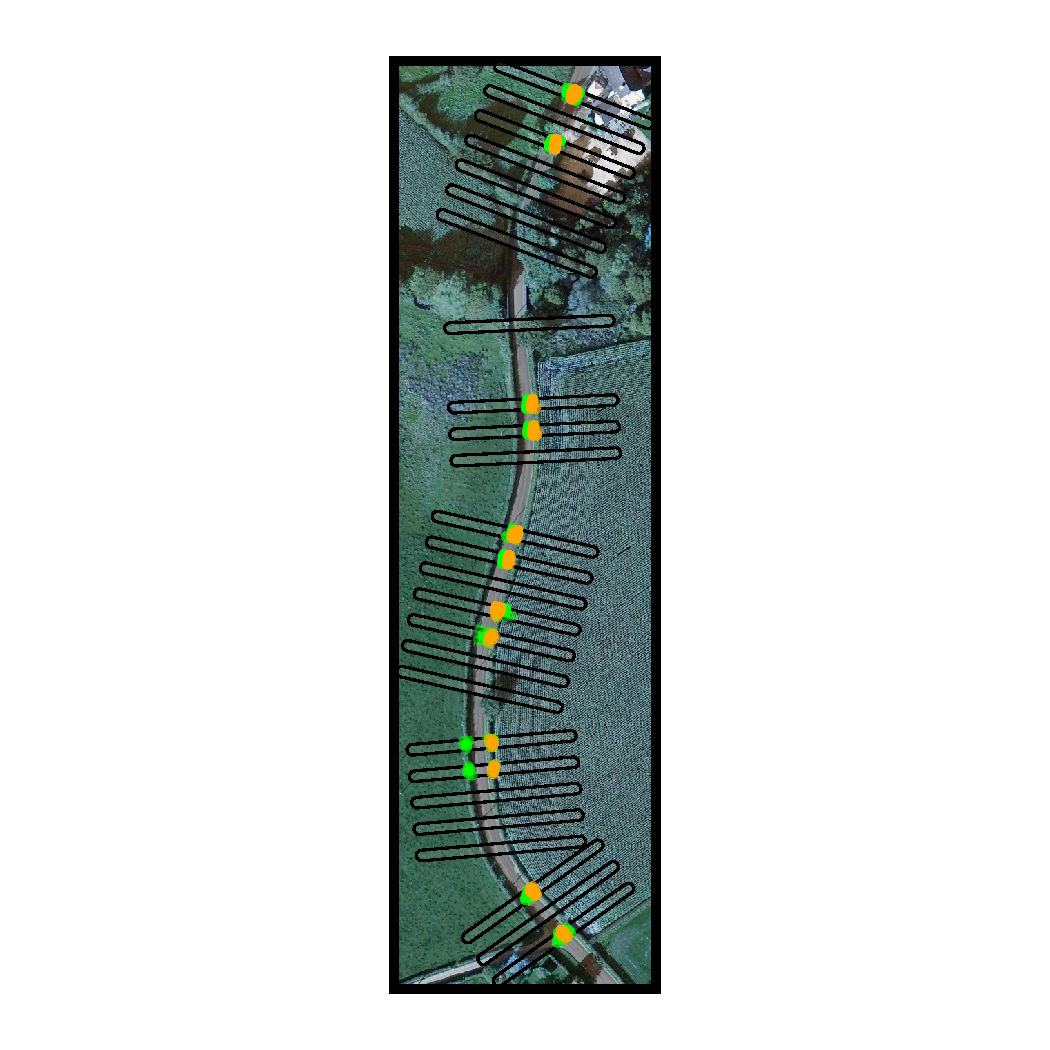
\includegraphics[width=\linewidth]{figure/lm_figs-1} 

}



\end{knitrout}



\begin{equation}
\begin{aligned}
\mathrm{Road}_{t} = \alpha 
    &+ \beta_{1}  \mathrm{Intensity}_{t} \\
    &+ \beta_{2}  \mathrm{Luminescence}_{t}    \\
    &+ \beta_{3}  \mathrm{Z}_{t} \\
    &+ \beta_{4}  \mathrm{Dist}_{t} + \epsilon
\end{aligned}
\end{equation}

//for this section see 450 assess2, details on validation etc.

\section{Noise Filtering}


\begin{knitrout}\footnotesize
\definecolor{shadecolor}{rgb}{0.969, 0.969, 0.969}\color{fgcolor}

{\centering 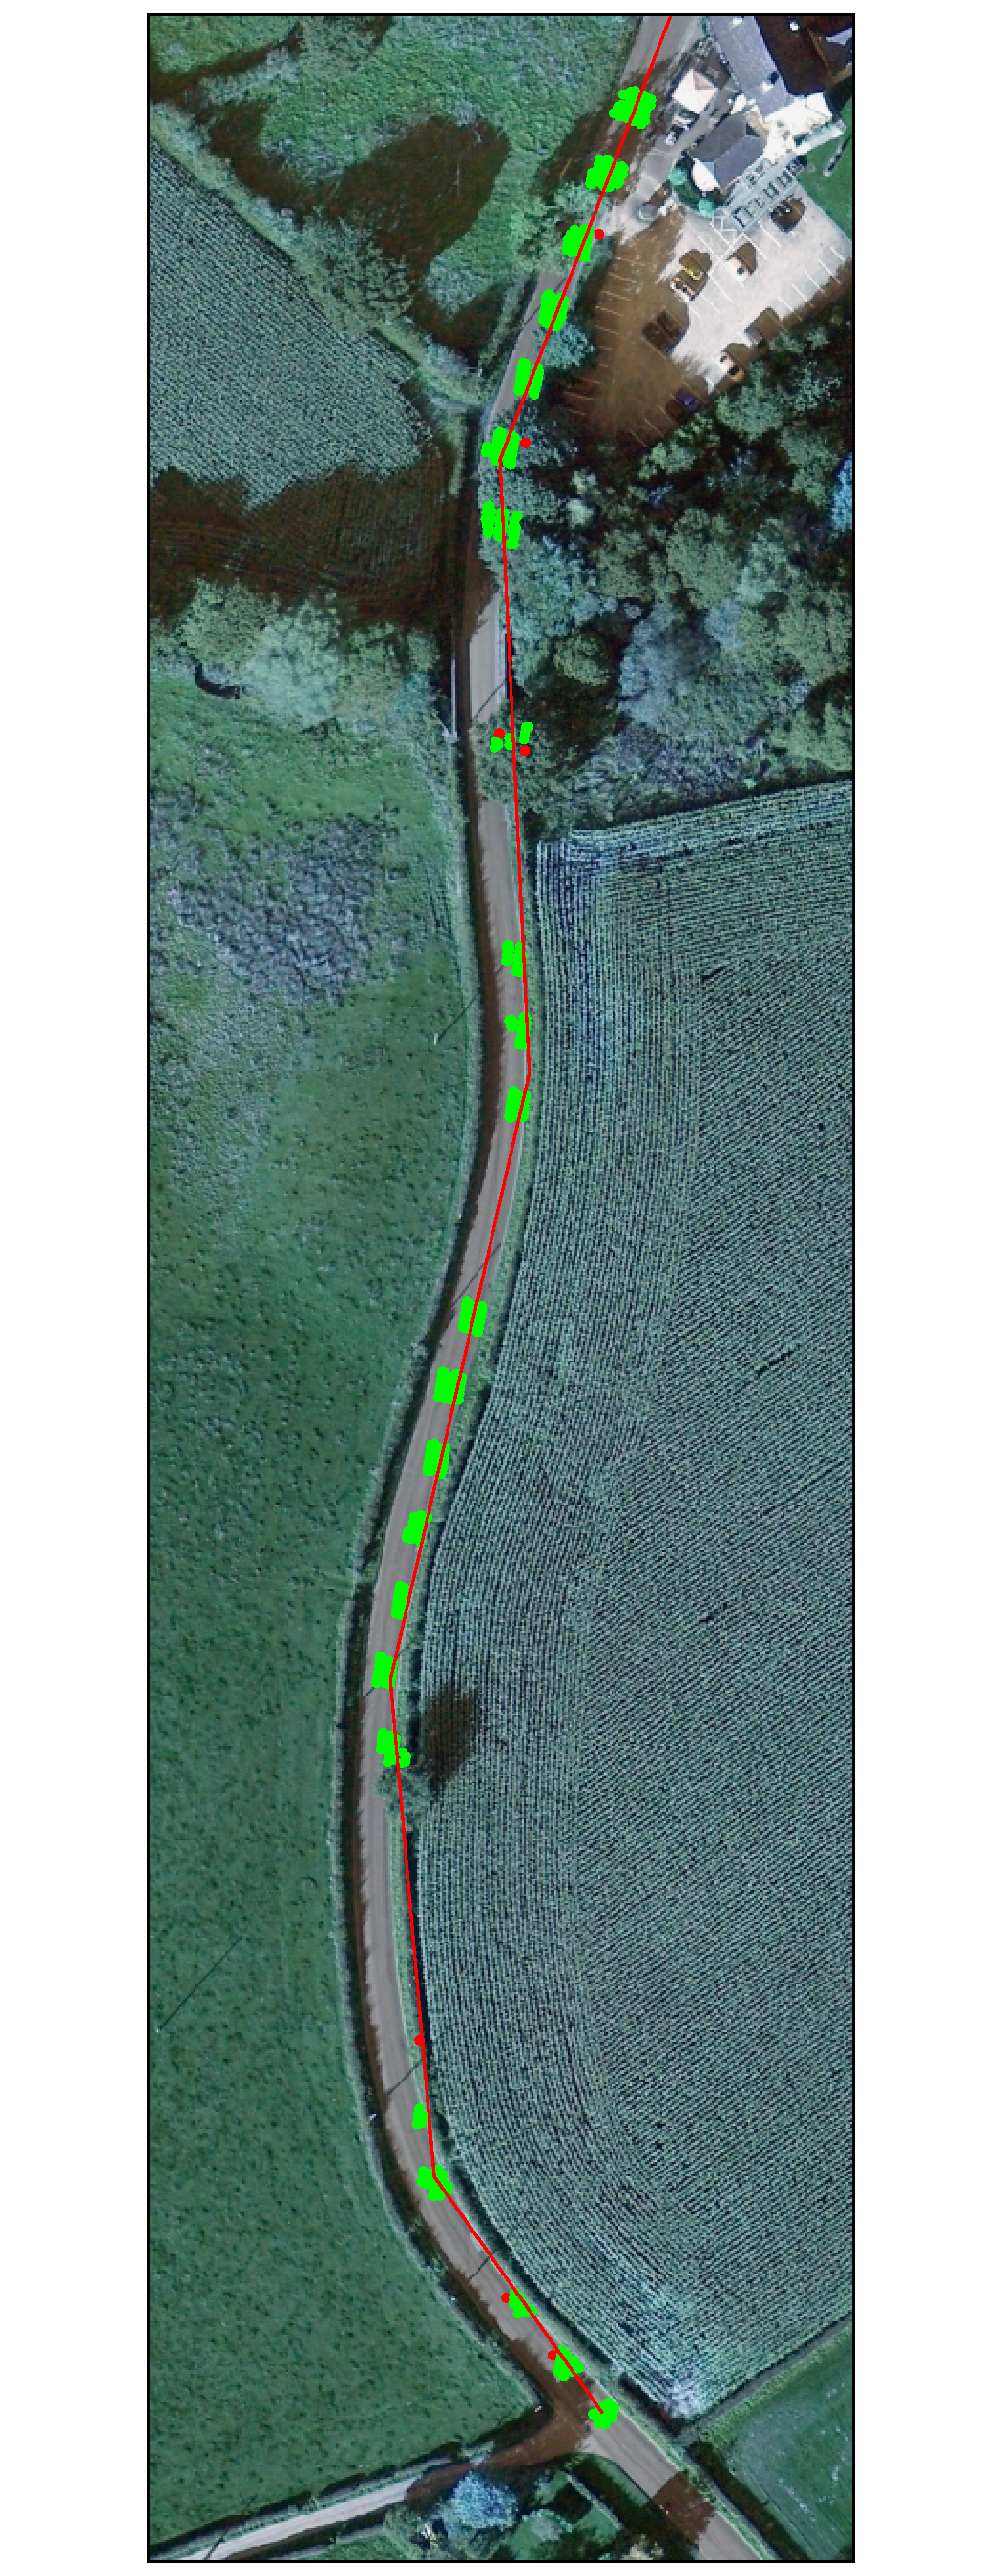
\includegraphics[width=\linewidth]{figure/fig_roadlines-1} 

}



\end{knitrout}

// Manually measure a road width for a reference, i.e. how close to accurate different models are. GLM LM and individual filtered and unfiltered. Find max and min widths and mean, describe what likely causes the differences.

\section{Final Model Analysis}

Very rough estimate of widths


\begin{table}[t]

\caption{\label{tab:mtest_tab}testing}
\centering
\fontsize{8}{10}\selectfont
\begin{tabular}{lr}
\toprule
\textbf{Model} & \textbf{Accuracy}\\
\midrule
lm 1 & 76.10\\
lm 2 & 77.72\\
lm 3 & 71.71\\
glm & 70.51\\
lm $i$ & 83.26\\
\bottomrule
\end{tabular}
\end{table}







\section{Road Assessment}


\begin{table}[H]

\caption{\label{tab:cor_table}Correlation Matrix}
\centering
\fontsize{8}{10}\selectfont
\begin{tabular}{lllll}
\toprule
\textbf{Variable} & \textbf{Width} & \textbf{Max Angle} & \textbf{Max Z} & \textbf{Int Range}\\
\midrule
Width &  & 0.22 & 0.44 & 0.32\\
Max Angle & 0.22 &  & 0.43 & 0.34\\
Max Z & 0.44 & 0.43 &  & 0.43\\
Int Range & 0.32 & 0.34 & 0.43 & \\
\bottomrule
\multicolumn{5}{l}{\textit{ }}\\
\multicolumn{5}{l}{*** Significant at the 0.001 level}\\
\multicolumn{5}{l}{** Significant at the 0.005 level}\\
\multicolumn{5}{l}{* Significant as the 0.01 level}\\
\end{tabular}
\end{table}



\begin{knitrout}\footnotesize
\definecolor{shadecolor}{rgb}{0.969, 0.969, 0.969}\color{fgcolor}

{\centering 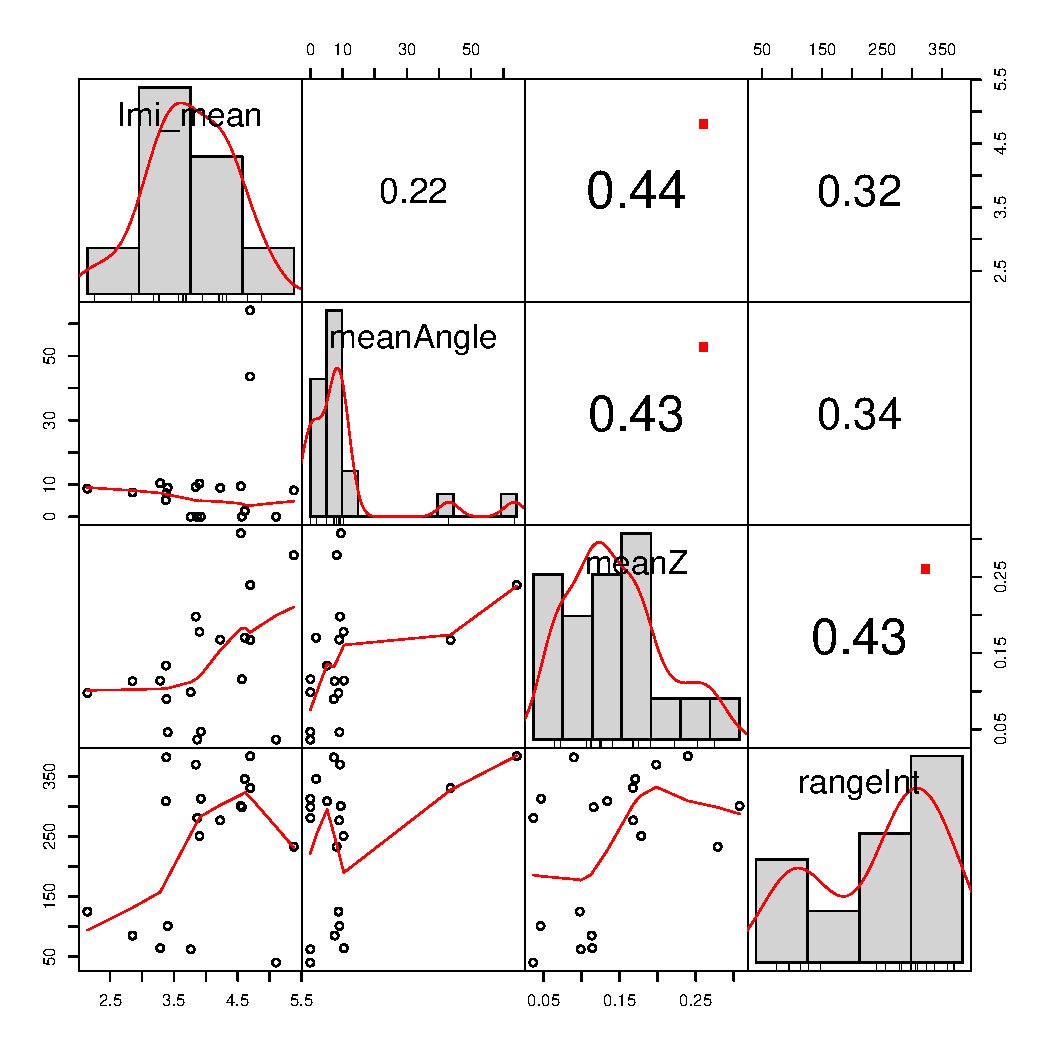
\includegraphics[width=\linewidth]{figure/unnamed-chunk-12-1} 

}



\end{knitrout}


\section{Widths and Road Quality}

\section{Road Analysis}

// if there is time:

Use width and max bend sharpness to estimate required speed for required stopping distance. Some maths could be involved. Use to produce speed limit assessment, include steepness somehow (speed limits due to stwwpwnss etc)

\end{multicols}

\chapter{Discussion}
\label{ch:discussion}

\begin{multicols}{2}
=== notes ===
\citep{hatger2005}
The idea now is to use this information in a more sensitive
segmentation, trying to extract the true road extents.
Of course, when there is no C0 (height) or C1 (inclination)
discontinuity at the road boundaries, there is no way de-
tecting it using laser scan data, and other data sources such
as aerial images have to be used. However, the question
is how reliable even small discontinuities can be detected.
For example, a road may be bounded by an embankment,
which usually is a relatively large structure. It may on the
other hand be separated from the pavement or a traffic is-
land by a kerb of only 15 cm in height. This seems to
be hopeless, since it is close to the expected noise of the
laser measurement. However, if one considers profiles per-
pendicular to the road, the point is that a 10 m wide road,
scanned with 1 m density, will yield 10 measurements to
estimate the road surface (assumed to be planar), leading
to a standard deviation of about 15 cm /
10  5 cm.

Assessment strategy: assessing the results of an image processing work flow usually a textual description. but results can't be compared easily. Heipke1997 sugest a comparison between methods numerically, ratios derived from statistical test theory:

be identiged.
True positive (TP) – A phenomenon that is present within the input data and that has
successfully been identiged within the output data.
False positive (FP) – A phenomenon that is not present within the input data but that
has falsely been found to be a phenomenon by the algorithm. Thus it is
written to output data.
False negative (FN) – A phenomenon that is present within the input data but that
has not been identiged by the algorithm and therefore has been omitted
from the output data.
Then we degne Completeness by
Completeness =
TP
.
TP + FN
(2.1)
This is obvious and can directly be taken from degnition of TP and FN.
Furthermore we degne Correctness by
Correctness =
TP
.
TP + FP
(2.2)
This is easy to see since we expect results not to contain features which are erroneous in
a way that they contain features which are not present within input data. However, it
is implied within this statement that we neglect those cases where features are present
within the input data but are missing in the output. Finally Quality is degned by
Quality =
TP
.
TP + FP + FN
(2.3)
This can be considered as a kind of global measure for overall assessment of obtained
results. It comprises e ects caused by both false positives and false negatives.
Some but not all of the algorithms investigated in this paper use an assessment that is
based on the above mentioned measures. Their results are reproduced where available.
Otherwise, assessment is done by means of a textual description.


// Mention logistic regression, considered but not used as results not better and requries a payoff.
\end{multicols}

\chapter{Conclusion}
\label{ch:conclusion}

\begin{multicols}{2}

\end{multicols}{2}

% ===========================================================================================================
% Bibliography
% ===========================================================================================================

\bibliographystyle{agsm}
\linespread{1}

\bibliography{kbib}

\begin{center}
% remember to compile twice for current word count
Word Count: 7224

\end{center}

\thispagestyle{newchapter}
\cleardoublepage

% ===========================================================================================================
% Appendices
% ===========================================================================================================
\appendix

\chapter{Code Appendix}
\label{a:code}

\section{Session Information}
\begin{knitrout}\footnotesize
\definecolor{shadecolor}{rgb}{0.969, 0.969, 0.969}\color{fgcolor}\begin{kframe}
\begin{verbatim}
Machine:     
\end{verbatim}


{\ttfamily\noindent\bfseries\color{errorcolor}{Error in get\_cpu(): could not find function "{}get\_cpu"{}}}\begin{verbatim}
Num cores:   
\end{verbatim}


{\ttfamily\noindent\bfseries\color{errorcolor}{Error in detectCores(logical = FALSE): could not find function "{}detectCores"{}}}\begin{verbatim}
Num threads: 
\end{verbatim}


{\ttfamily\noindent\bfseries\color{errorcolor}{Error in detectCores(logical = TRUE): could not find function "{}detectCores"{}}}\begin{verbatim}
RAM:         
\end{verbatim}


{\ttfamily\noindent\bfseries\color{errorcolor}{Error in get\_ram(): could not find function "{}get\_ram"{}}}\end{kframe}
\begin{kframe}\begin{verbatim}
R version 3.6.1 (2019-07-05)
Platform: x86_64-pc-linux-gnu (64-bit)
Running under: Manjaro Linux

Matrix products: default
BLAS:   /usr/lib/libopenblasp-r0.3.6.so
LAPACK: /usr/lib/liblapack.so.3.8.0

attached base packages:
[1] stats     graphics  grDevices utils     datasets  methods   base     

other attached packages:
 [1] pbapply_1.4-1              rgdal_1.4-4               
 [3] future_1.14.0              varhandle_2.0.3           
 [5] forcats_0.4.0              stringr_1.4.0             
 [7] dplyr_0.8.3                purrr_0.3.2               
 [9] readr_1.3.1                tidyr_0.8.3               
[11] tibble_2.1.3               tidyverse_1.2.1           
[13] lidR_2.1.2                 raster_2.9-23             
[15] sp_1.3-1                   scales_1.0.0              
[17] kableExtra_1.1.0           data.table_1.12.2         
[19] sf_0.7-7                   ggpubr_0.2.2              
[21] magrittr_1.5               cowplot_1.0.0             
[23] viridis_0.5.1              viridisLite_0.3.0         
[25] broom_0.5.2                ggthemes_4.2.0            
[27] RStoolbox_0.2.6            PerformanceAnalytics_1.5.3
[29] xts_0.11-2                 zoo_1.8-6                 
[31] Hmisc_4.2-0                ggplot2_3.2.0             
[33] Formula_1.2-3              survival_2.44-1.1         
[35] lattice_0.20-38            devtools_2.1.0            
[37] usethis_1.5.1              pacman_0.5.1              
[39] knitr_1.24                 nvimcom_0.9-83            
[41] colorout_1.2-1            
\end{verbatim}
\end{kframe}
\end{knitrout}
\newpage

\section{Functions}

\subsection{Formatting} \label{code:make_table}
\begin{knitrout}\footnotesize
\definecolor{shadecolor}{rgb}{0.969, 0.969, 0.969}\color{fgcolor}\begin{kframe}
\begin{alltt}
\hlstd{make_table} \hlkwb{<-} \hlkwa{function}\hlstd{(}\hlkwc{df}\hlstd{,} \hlkwc{cap}\hlstd{,} \hlkwc{dig} \hlstd{=} \hlnum{2}\hlstd{,} \hlkwc{...}\hlstd{) \{}
  \hlkwd{require}\hlstd{(kableExtra)}
  \hlkwd{require}\hlstd{(tidyverse)}

  \hlkwd{options}\hlstd{(}\hlkwc{knitr.kable.NA} \hlstd{=} \hlstr{""}\hlstd{)}
  \hlkwd{kable}\hlstd{(df,}
    \hlkwc{digits} \hlstd{= dig,} \hlkwc{caption} \hlstd{= cap,}
    \hlkwc{linesep} \hlstd{=} \hlstr{""}\hlstd{,}
    \hlkwc{longtable} \hlstd{=} \hlnum{FALSE}\hlstd{,} \hlkwc{booktabs} \hlstd{=} \hlnum{TRUE}\hlstd{,}
    \hlkwc{format} \hlstd{=} \hlstr{"latex"}\hlstd{,}
    \hlkwc{escape} \hlstd{= F}
  \hlstd{)} \hlopt
    \hlkwd{kable_styling}\hlstd{(}\hlkwc{font_size} \hlstd{=} \hlnum{8}\hlstd{)}  \hlopt
    \hlkwd{row_spec}\hlstd{(}\hlnum{0}\hlstd{,} \hlkwc{bold} \hlstd{=} \hlnum{TRUE}\hlstd{)}
\hlstd{\}}
\end{alltt}
\end{kframe}
\end{knitrout}
\subsection{Catalog to Dataframe} \label{code:ctg_to_df}
\begin{knitrout}\footnotesize
\definecolor{shadecolor}{rgb}{0.969, 0.969, 0.969}\color{fgcolor}\begin{kframe}
\begin{alltt}
\hlstd{ctg_to_df} \hlkwb{<-} \hlkwa{function}\hlstd{(}\hlkwc{cluster}\hlstd{) \{}
  \hlstd{las} \hlkwb{<-} \hlkwd{readLAS}\hlstd{(cluster)}
  \hlkwa{if} \hlstd{(}\hlkwd{is.empty}\hlstd{(las)) \{}
    \hlkwd{return}\hlstd{(}\hlkwa{NULL}\hlstd{)}
  \hlstd{\}}
  \hlstd{las} \hlkwb{<-} \hlkwd{as.spatial}\hlstd{(las)}
  \hlstd{las} \hlkwb{<-} \hlkwd{as.data.frame}\hlstd{(las)}
  \hlkwd{return}\hlstd{(las)}
\hlstd{\}}
\end{alltt}
\end{kframe}
\end{knitrout}

\subsection{Clip Samples} \label{code:clip_samples}
\begin{knitrout}\footnotesize
\definecolor{shadecolor}{rgb}{0.969, 0.969, 0.969}\color{fgcolor}\begin{kframe}
\begin{alltt}
\hlstd{clip_samples} \hlkwb{<-} \hlkwa{function}\hlstd{(}\hlkwc{cluster}\hlstd{,} \hlkwc{x}\hlstd{) \{}
  \hlstd{las} \hlkwb{<-} \hlkwd{readLAS}\hlstd{(cluster)}
  \hlkwa{if} \hlstd{(}\hlkwd{is.empty}\hlstd{(las)) \{}
    \hlkwd{return}\hlstd{(}\hlkwa{NULL}\hlstd{)}
  \hlstd{\}}
  \hlstd{las} \hlkwb{<-} \hlstd{las} \hlopt
    \hlkwd{as.spatial}\hlstd{()} \hlopt
    \hlkwd{st_as_sf}\hlstd{(las)} \hlopt
    \hlkwd{st_set_crs}\hlstd{(}\hlnum{27700}\hlstd{)} \hlopt
    \hlkwd{st_join}\hlstd{(x)}

  \hlstd{las} \hlkwb{<-} \hlstd{las[}\hlkwd{is.na}\hlstd{(las}\hlopt{$}\hlstd{sample_id)} \hlopt{==} \hlnum{FALSE}\hlstd{, ]}
  \hlkwd{return}\hlstd{(las)}
\hlstd{\}}
\end{alltt}
\end{kframe}
\end{knitrout}

\subsection{LiDAR Clean} \label{code:lidr_clean}
\begin{knitrout}\footnotesize
\definecolor{shadecolor}{rgb}{0.969, 0.969, 0.969}\color{fgcolor}\begin{kframe}
\begin{alltt}
\hlstd{lidr_clean} \hlkwb{<-} \hlkwa{function}\hlstd{(}\hlkwc{cluster}\hlstd{) \{}
  \hlstd{las} \hlkwb{<-} \hlkwd{readLAS}\hlstd{(cluster)}
  \hlkwa{if} \hlstd{(}\hlkwd{is.empty}\hlstd{(las)) \{}
    \hlkwd{return}\hlstd{(}\hlkwa{NULL}\hlstd{)}
  \hlstd{\}}
  \hlkwd{epsg}\hlstd{(las)} \hlkwb{<-} \hlnum{27700}
  \hlcom{# remove all but last return}
  \hlstd{las} \hlkwb{<-} \hlkwd{lasfilter}\hlstd{(las, NumberOfReturns} \hlopt{==} \hlstd{ReturnNumber)}

  \hlcom{# find ground points}
  \hlstd{las} \hlkwb{<-} \hlkwd{lasground}\hlstd{(las,} \hlkwd{csf}\hlstd{())}

  \hlcom{## Create Point DEM}
  \hlcom{# interpolate ground points to create raster dtm. Uses Classification = 2}
  \hlcom{# very large number of points, therefore idw used as opposed to kriging}
  \hlstd{dtm} \hlkwb{<-} \hlkwd{grid_terrain}\hlstd{(las,} \hlnum{1}\hlstd{,} \hlkwd{knnidw}\hlstd{(}\hlkwc{k} \hlstd{=} \hlnum{10}\hlstd{,} \hlkwc{p} \hlstd{=} \hlnum{2}\hlstd{))}
  \hlcom{# normalise heights using dtm}
  \hlstd{las} \hlkwb{<-} \hlkwd{lasnormalize}\hlstd{(las, dtm)}
  \hlkwd{return}\hlstd{(las)}
\hlstd{\}}
\end{alltt}
\end{kframe}
\end{knitrout}


\subsection{Extract Buffer} \label{code:extract_buff}
\begin{knitrout}\footnotesize
\definecolor{shadecolor}{rgb}{0.969, 0.969, 0.969}\color{fgcolor}\begin{kframe}
\begin{alltt}
\hlstd{extract_buff} \hlkwb{<-} \hlkwa{function}\hlstd{(}\hlkwc{cluster}\hlstd{,} \hlkwc{clip_input}\hlstd{) \{}
  \hlstd{las} \hlkwb{<-} \hlkwd{readLAS}\hlstd{(cluster)}

  \hlkwa{if} \hlstd{(}\hlkwd{is.empty}\hlstd{(las)) \{}
    \hlkwd{return}\hlstd{(}\hlkwa{NULL}\hlstd{)}
  \hlstd{\}}

  \hlkwa{if} \hlstd{(}\hlopt{!}\hlkwd{is.null}\hlstd{(clip_input)) \{}
    \hlstd{las} \hlkwb{<-} \hlkwd{lasclip}\hlstd{(las, clip_input)}

    \hlkwa{if} \hlstd{(}\hlkwd{length}\hlstd{(las)} \hlopt{>} \hlnum{1}\hlstd{) \{}
      \hlkwa{for} \hlstd{(i} \hlkwa{in} \hlnum{1}\hlopt{:}\hlkwd{length}\hlstd{(las)) \{}
        \hlkwa{if} \hlstd{(}\hlopt{!}\hlkwd{is.empty}\hlstd{(las[[i]])) \{}
          \hlstd{las} \hlkwb{<-} \hlkwd{do.call}\hlstd{(rbind, las)}
          \hlkwd{return}\hlstd{(las)}
        \hlstd{\}}
      \hlstd{\}}
    \hlstd{\}}
  \hlstd{\}}
\hlstd{\}}
\end{alltt}
\end{kframe}
\end{knitrout}

\subsection{Find Distances} \label{code:find_dists}
\begin{knitrout}\footnotesize
\definecolor{shadecolor}{rgb}{0.969, 0.969, 0.969}\color{fgcolor}\begin{kframe}
\begin{alltt}
\hlstd{find_dists} \hlkwb{<-} \hlkwa{function}\hlstd{(}\hlkwc{x}\hlstd{,} \hlkwc{y}\hlstd{) \{}
  \hlstd{d} \hlkwb{<-} \hlkwd{st_distance}\hlstd{(x, y)}
  \hlkwd{return}\hlstd{(d)}
\hlstd{\}}
\end{alltt}
\end{kframe}
\end{knitrout}

\subsection{Euclidean Distance} \label{code:euc}
\begin{knitrout}\footnotesize
\definecolor{shadecolor}{rgb}{0.969, 0.969, 0.969}\color{fgcolor}\begin{kframe}
\begin{alltt}
\hlcom{# Function to calculate Euclidean distance between 2 points}
\hlstd{euclidean_distance} \hlkwb{<-} \hlkwa{function}\hlstd{(}\hlkwc{p1}\hlstd{,} \hlkwc{p2}\hlstd{) \{}
  \hlkwd{return}\hlstd{(}\hlkwd{sqrt}\hlstd{((p2[}\hlnum{1}\hlstd{]} \hlopt{-} \hlstd{p1[}\hlnum{1}\hlstd{])}\hlopt{**}\hlnum{2} \hlopt{+} \hlstd{(p2[}\hlnum{2}\hlstd{]} \hlopt{-} \hlstd{p1[}\hlnum{2}\hlstd{])}\hlopt{**}\hlnum{2}\hlstd{))}
\hlstd{\}}
\end{alltt}
\end{kframe}
\end{knitrout}

\subsection{Perpendicular Sampling} \label{code:perp}
\begin{knitrout}\footnotesize
\definecolor{shadecolor}{rgb}{0.969, 0.969, 0.969}\color{fgcolor}\begin{kframe}
\begin{alltt}
\hlcom{# Function to calculate 2 points on a line perpendicular to another defined by 2 points p1,p2}
\hlcom{# For point at interval, which can be a proportion of the segment length, or a constant}
\hlcom{# At distance n from the source line}
\hlstd{calc_perp} \hlkwb{<-} \hlkwa{function}\hlstd{(}\hlkwc{p1}\hlstd{,} \hlkwc{p2}\hlstd{,} \hlkwc{n}\hlstd{,} \hlkwc{interval} \hlstd{=} \hlnum{0.5}\hlstd{,} \hlkwc{proportion} \hlstd{=} \hlnum{TRUE}\hlstd{) \{}
  \hlcom{# Calculate x and y distances}
  \hlstd{x_len} \hlkwb{<-} \hlstd{p2[}\hlnum{1}\hlstd{]} \hlopt{-} \hlstd{p1[}\hlnum{1}\hlstd{]}
  \hlstd{y_len} \hlkwb{<-} \hlstd{p2[}\hlnum{2}\hlstd{]} \hlopt{-} \hlstd{p1[}\hlnum{2}\hlstd{]}

  \hlcom{# If proportion calculate reference point from tot_length}
  \hlkwa{if} \hlstd{(proportion) \{}
    \hlstd{point} \hlkwb{<-} \hlkwd{c}\hlstd{(p1[}\hlnum{1}\hlstd{]} \hlopt{+} \hlstd{x_len} \hlopt{*} \hlstd{interval, p1[}\hlnum{2}\hlstd{]} \hlopt{+} \hlstd{y_len} \hlopt{*} \hlstd{interval)}
  \hlstd{\}}
  \hlcom{# Else use the constant value}
  \hlkwa{else} \hlstd{\{}
    \hlstd{tot_len} \hlkwb{<-} \hlkwd{euclidean_distance}\hlstd{(p1, p2)}
    \hlstd{point} \hlkwb{<-} \hlkwd{c}\hlstd{(}
      \hlstd{p1[}\hlnum{1}\hlstd{]} \hlopt{+} \hlstd{x_len} \hlopt{/} \hlstd{tot_len} \hlopt{*} \hlstd{interval,}
      \hlstd{p1[}\hlnum{2}\hlstd{]} \hlopt{+} \hlstd{y_len} \hlopt{/} \hlstd{tot_len} \hlopt{*} \hlstd{interval}
    \hlstd{)}
  \hlstd{\}}

  \hlcom{# Calculate the x and y distances from reference point}
  \hlcom{# to point on line n distance away}
  \hlstd{ref_len} \hlkwb{<-} \hlkwd{euclidean_distance}\hlstd{(point, p2)}
  \hlstd{xn_len} \hlkwb{<-} \hlstd{(n} \hlopt{/} \hlstd{ref_len)} \hlopt{*} \hlstd{(p2[}\hlnum{1}\hlstd{]} \hlopt{-} \hlstd{point[}\hlnum{1}\hlstd{])}
  \hlstd{yn_len} \hlkwb{<-} \hlstd{(n} \hlopt{/} \hlstd{ref_len)} \hlopt{*} \hlstd{(p2[}\hlnum{2}\hlstd{]} \hlopt{-} \hlstd{point[}\hlnum{2}\hlstd{])}

  \hlcom{# Invert the x and y lengths and add/subtract from the refrence point}
  \hlstd{ref_points} \hlkwb{<-} \hlkwd{rbind}\hlstd{(}
    \hlstd{point,}
    \hlkwd{c}\hlstd{(point[}\hlnum{1}\hlstd{]} \hlopt{+} \hlstd{yn_len, point[}\hlnum{2}\hlstd{]} \hlopt{-} \hlstd{xn_len),}
    \hlkwd{c}\hlstd{(point[}\hlnum{1}\hlstd{]} \hlopt{-} \hlstd{yn_len, point[}\hlnum{2}\hlstd{]} \hlopt{+} \hlstd{xn_len)}
  \hlstd{)}

  \hlcom{# Return the reference points}
  \hlkwd{return}\hlstd{(ref_points)}
\hlstd{\}}
\end{alltt}
\end{kframe}
\end{knitrout}

\subsection{Combine Catalog} \label{code:comb_ctg}
\begin{knitrout}\footnotesize
\definecolor{shadecolor}{rgb}{0.969, 0.969, 0.969}\color{fgcolor}\begin{kframe}
\begin{alltt}
\hlstd{comb_ctg} \hlkwb{<-} \hlkwa{function}\hlstd{(}\hlkwc{x}\hlstd{) \{}
  \hlstd{las} \hlkwb{<-} \hlkwd{readLAS}\hlstd{(x)}
  \hlkwa{if} \hlstd{(}\hlkwd{is.empty}\hlstd{(las)) \{}
    \hlkwd{return}\hlstd{(}\hlkwa{NULL}\hlstd{)}
  \hlstd{\}}
  \hlkwd{return}\hlstd{(las)}
\hlstd{\}}
\end{alltt}
\end{kframe}
\end{knitrout}

\subsection{Compute Samples} \label{code:compute_samples}
\begin{knitrout}\footnotesize
\definecolor{shadecolor}{rgb}{0.969, 0.969, 0.969}\color{fgcolor}\begin{kframe}
\begin{alltt}
\hlstd{sample_lines} \hlkwb{<-} \hlkwd{c}\hlstd{()}
\hlstd{compute_samples} \hlkwb{<-} \hlkwa{function}\hlstd{(}\hlkwc{x}\hlstd{) \{}
  \hlkwa{if} \hlstd{(}\hlkwd{nrow}\hlstd{(x)} \hlopt{>} \hlnum{1}\hlstd{) \{}
    \hlstd{road_node} \hlkwb{<-} \hlkwd{st_coordinates}\hlstd{(x)}
    \hlstd{tot_len} \hlkwb{<-} \hlnum{0}
    \hlstd{len_inc} \hlkwb{<-} \hlnum{10}
    \hlstd{len_ofs} \hlkwb{<-} \hlstd{len_inc}
    \hlkwa{for} \hlstd{(i} \hlkwa{in} \hlnum{2}\hlopt{:}\hlkwd{nrow}\hlstd{(road_node)} \hlopt{-} \hlnum{1}\hlstd{) \{}
      \hlstd{n1} \hlkwb{<-} \hlstd{road_node[i, ]}
      \hlstd{n2} \hlkwb{<-} \hlstd{road_node[i} \hlopt{+} \hlnum{1}\hlstd{, ]}

      \hlstd{len_seg} \hlkwb{<-} \hlkwd{euclidean_distance}\hlstd{(n1, n2)}
      \hlstd{len_ofs} \hlkwb{<-} \hlstd{len_ofs} \hlopt{+} \hlstd{len_inc}

      \hlkwa{while} \hlstd{(len_ofs} \hlopt{<=} \hlstd{tot_len} \hlopt{+} \hlstd{len_seg) \{}
        \hlstd{len_ofs} \hlkwb{<-} \hlstd{len_ofs} \hlopt{+} \hlstd{len_inc}

        \hlcom{# Add results to output vector}
        \hlstd{perp_segments} \hlkwb{<-} \hlkwd{calc_perp}\hlstd{(}
          \hlstd{n1, n2,} \hlnum{30}\hlstd{,}
          \hlstd{len_ofs} \hlopt{-} \hlstd{tot_len,}
          \hlkwc{proportion} \hlstd{=} \hlnum{FALSE}
        \hlstd{)}

        \hlstd{multipoints} \hlkwb{<-} \hlkwd{st_multipoint}\hlstd{(}\hlkwd{matrix}\hlstd{(perp_segments,} \hlkwc{ncol} \hlstd{=} \hlnum{2}\hlstd{))}
        \hlstd{pts} \hlkwb{<-} \hlkwd{st_cast}\hlstd{(}\hlkwd{st_geometry}\hlstd{(multipoints),} \hlstr{"POINT"}\hlstd{)}
        \hlstd{n} \hlkwb{<-} \hlkwd{length}\hlstd{(pts)}

        \hlstd{pair} \hlkwb{<-} \hlkwd{st_combine}\hlstd{(}\hlkwd{c}\hlstd{(pts[}\hlnum{1}\hlstd{], pts[}\hlnum{2}\hlstd{], pts[}\hlnum{3}\hlstd{]))}
        \hlstd{linestring} \hlkwb{<-} \hlkwd{st_cast}\hlstd{(pair,} \hlstr{"LINESTRING"}\hlstd{)} \hlopt
          \hlkwd{st_buffer}\hlstd{(}\hlnum{2}\hlstd{)} \hlopt
          \hlkwd{st_sf}\hlstd{()} \hlopt
          \hlkwd{mutate}\hlstd{(}\hlkwc{road_id} \hlstd{=} \hlkwd{as.character}\hlstd{(}\hlkwd{unique}\hlstd{(x}\hlopt{$}\hlstd{road_id)))}
        \hlstd{sample_lines} \hlkwb{<-} \hlkwd{rbind}\hlstd{(sample_lines, linestring)}
      \hlstd{\}}
      \hlstd{tot_len} \hlkwb{<-} \hlstd{tot_len} \hlopt{+} \hlstd{len_seg}
    \hlstd{\}}
  \hlstd{\}}
  \hlkwd{return}\hlstd{(sample_lines)}
\hlstd{\}}
\end{alltt}
\end{kframe}
\end{knitrout}

\subsection{Greyscale} \label{code:greyscale}
\begin{knitrout}\footnotesize
\definecolor{shadecolor}{rgb}{0.969, 0.969, 0.969}\color{fgcolor}\begin{kframe}
\begin{alltt}
\hlstd{greyscale} \hlkwb{<-} \hlkwa{function}\hlstd{(}\hlkwc{x}\hlstd{) \{}
  \hlstd{x} \hlkwb{<-} \hlstd{(x[[}\hlnum{1}\hlstd{]]} \hlopt{+} \hlstd{x[[}\hlnum{2}\hlstd{]]} \hlopt{+} \hlstd{x[[}\hlnum{3}\hlstd{]])} \hlopt{/} \hlnum{3}
\hlstd{\}}
\end{alltt}
\end{kframe}
\end{knitrout}

\subsection{Compute Individual Linear Model} \label{code:lm_compute}
\begin{knitrout}\footnotesize
\definecolor{shadecolor}{rgb}{0.969, 0.969, 0.969}\color{fgcolor}\begin{kframe}
\begin{alltt}
\hlstd{lm_compute} \hlkwb{<-} \hlkwa{function}\hlstd{(}\hlkwc{x}\hlstd{,} \hlkwc{f}\hlstd{)} \hlkwd{tryCatch}\hlstd{(\{}
    \hlstd{m} \hlkwb{<-} \hlkwd{lm}\hlstd{(}\hlkwc{formula} \hlstd{= f,} \hlkwc{data} \hlstd{= x)}

    \hlstd{p} \hlkwb{<-} \hlstd{m} \hlopt
      \hlkwd{tidy}\hlstd{()} \hlopt
      \hlstd{dplyr}\hlopt{::}\hlkwd{select}\hlstd{(}\hlkwc{p} \hlstd{= p.value)}

    \hlstd{pred_m} \hlkwb{<-} \hlkwd{predict}\hlstd{(m, x,} \hlkwc{type} \hlstd{=} \hlstr{"response"}\hlstd{)}

    \hlkwa{if} \hlstd{(}\hlkwd{sum}\hlstd{(p)} \hlopt{/} \hlkwd{nrow}\hlstd{(p)} \hlopt{<} \hlnum{0.05}\hlstd{) \{}
      \hlstd{x}\hlopt{$}\hlstd{lm} \hlkwb{<-} \hlstd{pred_m}
    \hlstd{\}} \hlkwa{else} \hlstd{\{}
      \hlstd{x}\hlopt{$}\hlstd{lm} \hlkwb{<-} \hlnum{NA}
    \hlstd{\}}

    \hlstd{x}\hlopt{$}\hlstd{lmI_dum} \hlkwb{<-} \hlkwd{ifelse}\hlstd{(x}\hlopt{$}\hlstd{lm} \hlopt{>} \hlkwd{quantile}\hlstd{(x}\hlopt{$}\hlstd{lm,} \hlnum{.95}\hlstd{),} \hlnum{1}\hlstd{,} \hlnum{0}\hlstd{)}
    \hlstd{x}\hlopt{$}\hlstd{lmI_dum} \hlkwb{<-} \hlkwd{ifelse}\hlstd{(x}\hlopt{$}\hlstd{lm} \hlopt{>} \hlkwd{quantile}\hlstd{(x}\hlopt{$}\hlstd{lm,} \hlnum{.95}\hlstd{),} \hlnum{1}\hlstd{,} \hlnum{0}\hlstd{)}
    \hlstd{x}\hlopt{$}\hlstd{p_val} \hlkwb{<-} \hlkwd{sum}\hlstd{(p)}

    \hlkwd{return}\hlstd{(x)}
  \hlstd{\},} \hlkwc{error} \hlstd{=} \hlkwa{function}\hlstd{(}\hlkwc{e}\hlstd{)} \hlkwa{NULL}\hlstd{)}
\end{alltt}
\end{kframe}
\end{knitrout}

\subsection{Filter Returns}
\begin{knitrout}\footnotesize
\definecolor{shadecolor}{rgb}{0.969, 0.969, 0.969}\color{fgcolor}\begin{kframe}
\begin{alltt}
\hlstd{filter_returns} \hlkwb{<-} \hlkwa{function}\hlstd{(}\hlkwc{x}\hlstd{) \{}
  \hlstd{road} \hlkwb{<-} \hlstd{x[x}\hlopt{$}\hlstd{road} \hlopt{==} \hlnum{1}\hlstd{, ]}
  \hlkwa{if} \hlstd{(}\hlkwd{max}\hlstd{(road}\hlopt{$}\hlstd{NumberOfReturns)} \hlopt{==} \hlnum{1}\hlstd{) \{}
    \hlkwd{return}\hlstd{(x)}
  \hlstd{\}}
\hlstd{\}}
\end{alltt}
\end{kframe}
\end{knitrout}

\subsection{Filter Samples}
\begin{knitrout}\footnotesize
\definecolor{shadecolor}{rgb}{0.969, 0.969, 0.969}\color{fgcolor}\begin{kframe}
\begin{alltt}
\hlstd{filter_samples} \hlkwb{<-} \hlkwa{function}\hlstd{(}\hlkwc{s}\hlstd{) \{}
  \hlcom{# find rows far below mean}
  \hlkwa{if} \hlstd{(}\hlkwd{nrow}\hlstd{(s)} \hlopt{>} \hlkwd{mean}\hlstd{(}\hlkwd{nrow}\hlstd{(s))} \hlopt{/} \hlnum{4}\hlstd{) \{}
    \hlcom{# remove outlier points}
    \hlstd{distances} \hlkwb{<-} \hlstd{s} \hlopt
      \hlkwd{st_distance}\hlstd{()} \hlopt
      \hlkwd{apply}\hlstd{(}\hlnum{1}\hlstd{,} \hlkwc{FUN} \hlstd{=} \hlkwa{function}\hlstd{(}\hlkwc{y}\hlstd{) \{}
        \hlkwd{min}\hlstd{(y[y} \hlopt{>} \hlnum{0}\hlstd{])}
      \hlstd{\})} \hlopt
      \hlkwd{as.data.frame}\hlstd{()} \hlopt
      \hlkwd{mutate}\hlstd{(}\hlkwc{rowid} \hlstd{=} \hlkwd{row_number}\hlstd{())} \hlopt
      \hlkwd{select}\hlstd{(}\hlkwc{min_dist} \hlstd{=} \hlstr{"."}\hlstd{, rowid)}

    \hlcom{# above 1m from any other point}
    \hlstd{distances} \hlkwb{<-} \hlstd{distances[distances}\hlopt{$}\hlstd{min_dist} \hlopt{<} \hlnum{1}\hlstd{, ]}

    \hlstd{s} \hlkwb{<-} \hlstd{s} \hlopt \hlkwd{mutate}\hlstd{(}\hlkwc{rowid} \hlstd{=} \hlkwd{row_number}\hlstd{())}

    \hlstd{s} \hlkwb{<-} \hlstd{s[s}\hlopt{$}\hlstd{rowid} \hlopt \hlstd{distances}\hlopt{$}\hlstd{rowid, ]}
    \hlkwd{return}\hlstd{(s)}
  \hlstd{\}}
\hlstd{\}}
\end{alltt}
\end{kframe}
\end{knitrout}

\subsection{Max Dist}
\begin{knitrout}\footnotesize
\definecolor{shadecolor}{rgb}{0.969, 0.969, 0.969}\color{fgcolor}\begin{kframe}
\begin{alltt}
\hlstd{max_dist} \hlkwb{<-} \hlkwa{function}\hlstd{(}\hlkwc{x}\hlstd{) \{}
  \hlstd{tot_dists} \hlkwb{<-} \hlkwd{c}\hlstd{()}
  \hlstd{distances} \hlkwb{<-} \hlstd{x} \hlopt
    \hlkwd{st_distance}\hlstd{(}\hlkwc{by_element} \hlstd{=} \hlnum{FALSE}\hlstd{)} \hlopt
    \hlkwd{unclass}\hlstd{()} \hlopt
    \hlstr{"[<-"}\hlstd{(}\hlkwd{lower.tri}\hlstd{(.,} \hlkwc{diag} \hlstd{=} \hlnum{TRUE}\hlstd{),} \hlnum{NA}\hlstd{)} \hlopt
    \hlkwd{as_tibble}\hlstd{()} \hlopt
    \hlkwd{rowid_to_column}\hlstd{()} \hlopt
    \hlkwd{gather}\hlstd{(colid, distance,} \hlkwd{starts_with}\hlstd{(}\hlstr{"V"}\hlstd{),}
      \hlkwc{na.rm} \hlstd{=} \hlnum{TRUE}
    \hlstd{)} \hlopt
    \hlkwd{arrange}\hlstd{(}\hlkwd{desc}\hlstd{(distance))}

  \hlkwa{if} \hlstd{(}\hlkwd{nrow}\hlstd{(distances)} \hlopt{>} \hlnum{0}\hlstd{) \{}
    \hlstd{distances}\hlopt{$}\hlstd{colid} \hlkwb{<-} \hlkwd{gsub}\hlstd{(}\hlstr{"[^0-9.-]"}\hlstd{,} \hlstr{""}\hlstd{, distances}\hlopt{$}\hlstd{colid)}
    \hlstd{tot_dists} \hlkwb{<-} \hlkwd{rbind}\hlstd{(tot_dists,} \hlkwd{max}\hlstd{(distances}\hlopt{$}\hlstd{distance))}

    \hlstd{distances} \hlkwb{<-} \hlkwd{as.list}\hlstd{(distances[}\hlnum{1}\hlstd{,} \hlnum{1}\hlopt{:}\hlnum{2}\hlstd{])} \hlopt
      \hlkwd{unlist}\hlstd{()} \hlopt
      \hlkwd{as.numeric}\hlstd{()}

    \hlstd{x} \hlkwb{<-} \hlstd{x[distances, ]} \hlopt
      \hlkwd{st_combine}\hlstd{()} \hlopt
      \hlkwd{st_sf}\hlstd{()} \hlopt
      \hlkwd{st_cast}\hlstd{(}\hlstr{"LINESTRING"}\hlstd{)}
    \hlkwd{return}\hlstd{(x)}
  \hlstd{\}}
\hlstd{\}}
\end{alltt}
\end{kframe}
\end{knitrout}

\subsection{Max Lines}
\begin{knitrout}\footnotesize
\definecolor{shadecolor}{rgb}{0.969, 0.969, 0.969}\color{fgcolor}\begin{kframe}
\begin{alltt}
\hlstd{max_lines} \hlkwb{<-} \hlkwa{function}\hlstd{(}\hlkwc{x}\hlstd{) \{}
  \hlstd{road_lm} \hlkwb{<-} \hlkwd{split}\hlstd{(x,} \hlkwc{f} \hlstd{= x}\hlopt{$}\hlstd{sample_id)}

  \hlstd{road_lm} \hlkwb{<-} \hlstd{road_lm} \hlopt \hlkwd{compact}\hlstd{()}

  \hlstd{road_lm} \hlkwb{<-} \hlkwd{lapply}\hlstd{(road_lm, filter_samples)}
  \hlstd{road_lm} \hlkwb{<-} \hlkwd{lapply}\hlstd{(road_lm, max_dist)}
  \hlstd{road_lm} \hlkwb{<-} \hlkwd{do.call}\hlstd{(rbind, road_lm)}
  \hlcom{# find intersecting buffers}
  \hlstd{road_lm} \hlkwb{<-} \hlkwd{st_join}\hlstd{(road_lm, road_buff)}

  \hlkwd{return}\hlstd{(road_lm)}
\hlstd{\}}

\hlcom{## -- model_comparison}
\hlstd{model_comparison} \hlkwb{<-} \hlkwa{function}\hlstd{(}\hlkwc{model}\hlstd{) \{}
  \hlstd{road_lm} \hlkwb{<-} \hlstd{model[}\hlopt{!}\hlkwd{is.na}\hlstd{(model}\hlopt{$}\hlstd{roadFunction), ]}
  \hlstd{rds} \hlkwb{<-} \hlkwd{unique}\hlstd{(model}\hlopt{$}\hlstd{road_id)}
  \hlstd{road_lm} \hlkwb{<-} \hlkwd{split}\hlstd{(road_lm,} \hlkwc{f} \hlstd{= road_lm}\hlopt{$}\hlstd{road_id)}

  \hlstd{samp} \hlkwb{<-} \hlkwd{Filter}\hlstd{(}\hlkwa{function}\hlstd{(}\hlkwc{x}\hlstd{)} \hlkwd{dim}\hlstd{(x)[}\hlnum{1}\hlstd{]} \hlopt{>} \hlnum{0}\hlstd{, road_lm)}
  \hlstd{cent} \hlkwb{<-} \hlstd{centrelines[centrelines}\hlopt{$}\hlstd{road_id} \hlopt \hlstd{rds, ]}
  \hlstd{cent} \hlkwb{<-} \hlkwd{split}\hlstd{(cent,} \hlkwc{f} \hlstd{= cent}\hlopt{$}\hlstd{road_id)}
  \hlstd{cent} \hlkwb{<-} \hlkwd{Filter}\hlstd{(}\hlkwa{function}\hlstd{(}\hlkwc{x}\hlstd{)} \hlkwd{dim}\hlstd{(x)[}\hlnum{1}\hlstd{]} \hlopt{>} \hlnum{0}\hlstd{, cent)}

  \hlcom{## ---- find true widths}
  \hlstd{widths} \hlkwb{<-} \hlkwd{mapply}\hlstd{(opposite_length, samp, cent)}
  \hlstd{widths} \hlkwb{<-} \hlkwd{do.call}\hlstd{(rbind, widths)}
  \hlstd{widths} \hlkwb{<-} \hlkwd{as.data.frame}\hlstd{(widths)}

  \hlstd{widths}\hlopt{$}\hlstd{opposite} \hlkwb{<-} \hlkwd{as.numeric}\hlstd{(}\hlkwd{unfactor}\hlstd{(widths}\hlopt{$}\hlstd{opposite))}

  \hlstd{widths} \hlkwb{<-} \hlstd{widths[widths}\hlopt{$}\hlstd{opposite} \hlopt{>} \hlnum{2} \hlopt{&} \hlstd{widths}\hlopt{$}\hlstd{opposite} \hlopt{<} \hlnum{8}\hlstd{, ]}

  \hlstd{widths} \hlkwb{<-} \hlstd{widths} \hlopt
    \hlkwd{group_by}\hlstd{(V2)} \hlopt
    \hlkwd{select}\hlstd{(}\hlkwc{road_id} \hlstd{= V2, opposite)} \hlopt
    \hlkwd{summarise}\hlstd{(}
      \hlkwc{mean_width} \hlstd{=} \hlkwd{mean}\hlstd{(opposite)}
    \hlstd{)}

  \hlkwd{return}\hlstd{(widths)}
\hlstd{\}}
\end{alltt}
\end{kframe}
\end{knitrout}

\subsection{Model Comparison}


\subsection{Opposite Length}
\begin{knitrout}\footnotesize
\definecolor{shadecolor}{rgb}{0.969, 0.969, 0.969}\color{fgcolor}\begin{kframe}
\begin{alltt}
\hlstd{opposite_length} \hlkwb{<-} \hlkwa{function}\hlstd{(}\hlkwc{samp}\hlstd{,} \hlkwc{cent}\hlstd{) \{}
  \hlstd{tot_width} \hlkwb{<-} \hlkwd{c}\hlstd{()}
  \hlstd{cent} \hlkwb{<-} \hlstd{cent} \hlopt \hlkwd{st_cast}\hlstd{(}\hlstr{"POINT"}\hlstd{)}
  \hlstd{n} \hlkwb{<-} \hlkwd{nrow}\hlstd{(cent)} \hlopt{-} \hlnum{1}
  \hlstd{nodelines} \hlkwb{<-} \hlkwd{lapply}\hlstd{(}\hlkwc{X} \hlstd{=} \hlnum{1}\hlopt{:}\hlstd{n,} \hlkwc{FUN} \hlstd{=} \hlkwa{function}\hlstd{(}\hlkwc{i}\hlstd{) \{}
    \hlstd{pair} \hlkwb{<-} \hlstd{cent[}\hlkwd{c}\hlstd{(i, i} \hlopt{+} \hlnum{1}\hlstd{), ]} \hlopt
      \hlkwd{st_combine}\hlstd{()}
    \hlstd{line} \hlkwb{<-} \hlkwd{st_cast}\hlstd{(pair,} \hlstr{"LINESTRING"}\hlstd{)}
    \hlkwd{return}\hlstd{(line)}
  \hlstd{\})}

  \hlstd{samp} \hlkwb{<-} \hlstd{samp} \hlopt
    \hlkwd{mutate}\hlstd{(}\hlkwc{row_id} \hlstd{=} \hlkwd{row_number}\hlstd{())}
  \hlstd{samp} \hlkwb{<-} \hlkwd{split}\hlstd{(samp, samp}\hlopt{$}\hlstd{row_id)}
  \hlkwa{for} \hlstd{(n} \hlkwa{in} \hlstd{nodelines) \{}
    \hlkwa{for} \hlstd{(s} \hlkwa{in} \hlstd{samp) \{}
      \hlstd{int} \hlkwb{<-} \hlkwd{as.numeric}\hlstd{(}\hlkwd{st_crosses}\hlstd{(n, s))}
      \hlstd{int[}\hlkwd{is.na}\hlstd{(int)]} \hlkwb{<-} \hlnum{0}
      \hlkwa{if} \hlstd{(int} \hlopt{==} \hlnum{1}\hlstd{) \{}
        \hlstd{n1} \hlkwb{<-} \hlkwd{st_coordinates}\hlstd{(n)[}\hlnum{1}\hlstd{, ]}
        \hlstd{n2} \hlkwb{<-} \hlkwd{st_coordinates}\hlstd{(n)[}\hlnum{2}\hlstd{, ]}
        \hlstd{x} \hlkwb{<-} \hlstd{n1[}\hlnum{1}\hlstd{]} \hlopt{-} \hlstd{n2[}\hlnum{1}\hlstd{]}
        \hlstd{y} \hlkwb{<-} \hlstd{n1[}\hlnum{2}\hlstd{]} \hlopt{-} \hlstd{n2[}\hlnum{2}\hlstd{]}
        \hlstd{ang_rad} \hlkwb{<-} \hlkwd{atan2}\hlstd{(x, y)}
        \hlstd{ang_deg} \hlkwb{<-} \hlstd{ang_rad} \hlopt{*} \hlnum{180} \hlopt{/} \hlstd{pi}
        \hlkwa{if} \hlstd{(ang_rad} \hlopt{<} \hlnum{0}\hlstd{) \{}
          \hlstd{ang_deg} \hlkwb{<-} \hlstd{ang_deg} \hlopt{+} \hlnum{180}
        \hlstd{\}}

        \hlstd{n1} \hlkwb{<-} \hlkwd{st_coordinates}\hlstd{(s)[}\hlnum{1}\hlstd{, ]}
        \hlstd{n2} \hlkwb{<-} \hlkwd{st_coordinates}\hlstd{(s)[}\hlnum{2}\hlstd{, ]}
        \hlstd{x} \hlkwb{<-} \hlstd{n1[}\hlnum{1}\hlstd{]} \hlopt{-} \hlstd{n2[}\hlnum{2}\hlstd{]}
        \hlstd{y} \hlkwb{<-} \hlstd{n1[}\hlnum{2}\hlstd{]} \hlopt{-} \hlstd{n2[}\hlnum{2}\hlstd{]}

        \hlstd{ang_rad} \hlkwb{<-} \hlkwd{atan2}\hlstd{(x, y)}
        \hlstd{ang_deg_c} \hlkwb{<-} \hlstd{ang_rad} \hlopt{*} \hlnum{180} \hlopt{/} \hlstd{pi}
        \hlkwa{if} \hlstd{(ang_rad} \hlopt{<} \hlnum{0}\hlstd{) \{}
          \hlstd{ang_deg_c} \hlkwb{<-} \hlstd{ang_deg} \hlopt{+} \hlnum{180}
        \hlstd{\}}

        \hlstd{theta} \hlkwb{<-} \hlstd{ang_deg} \hlopt{-} \hlstd{ang_deg_c}
        \hlstd{theta} \hlkwb{<-} \hlstd{theta} \hlopt{-} \hlnum{45} \hlcom{# position relation to perp line}

        \hlstd{c1_len} \hlkwb{<-} \hlkwd{st_length}\hlstd{(s)}
        \hlstd{opposite} \hlkwb{<-} \hlkwd{abs}\hlstd{(}\hlkwd{as.numeric}\hlstd{(c1_len)} \hlopt{*} \hlkwd{cos}\hlstd{(}\hlkwd{as.numeric}\hlstd{(theta)))}
        \hlstd{opposite} \hlkwb{<-} \hlkwd{cbind}\hlstd{(}
          \hlstd{opposite,} \hlkwd{as.character}\hlstd{(}\hlkwd{unique}\hlstd{(cent}\hlopt{$}\hlstd{road_id)),}
          \hlkwd{as.character}\hlstd{(}\hlkwd{unique}\hlstd{(cent}\hlopt{$}\hlstd{sample_id))}
        \hlstd{)}
        \hlstd{tot_width} \hlkwb{<-} \hlkwd{rbind}\hlstd{(tot_width, opposite)}
      \hlstd{\}}
    \hlstd{\}}
  \hlstd{\}}
  \hlkwd{return}\hlstd{(tot_width)}
\hlstd{\}}
\end{alltt}
\end{kframe}
\end{knitrout}

\subsection{Road Angles}
\begin{knitrout}\footnotesize
\definecolor{shadecolor}{rgb}{0.969, 0.969, 0.969}\color{fgcolor}\begin{kframe}
\begin{alltt}
\hlstd{road_angles} \hlkwb{<-} \hlkwa{function}\hlstd{(}\hlkwc{rd}\hlstd{) \{}
  \hlstd{coords} \hlkwb{<-} \hlstd{rd} \hlopt \hlkwd{st_coordinates}\hlstd{()}
  \hlstd{angle} \hlkwb{<-} \hlkwd{c}\hlstd{()}
  \hlkwa{if} \hlstd{(}\hlkwd{nrow}\hlstd{(coords)} \hlopt{>} \hlnum{1}\hlstd{) \{}
    \hlkwa{for} \hlstd{(i} \hlkwa{in} \hlnum{1}\hlopt{:}\hlstd{(}\hlkwd{nrow}\hlstd{(rd)} \hlopt{-} \hlnum{1}\hlstd{)) \{}
      \hlstd{n1} \hlkwb{<-} \hlstd{coords[i, ]}
      \hlstd{n2} \hlkwb{<-} \hlstd{coords[i} \hlopt{+} \hlnum{1}\hlstd{, ]}
      \hlstd{x} \hlkwb{<-} \hlstd{n1[}\hlnum{1}\hlstd{]} \hlopt{-} \hlstd{n2[}\hlnum{1}\hlstd{]}
      \hlstd{y} \hlkwb{<-} \hlstd{n1[}\hlnum{2}\hlstd{]} \hlopt{-} \hlstd{n2[}\hlnum{2}\hlstd{]}
      \hlstd{ang_rad} \hlkwb{<-} \hlkwd{atan2}\hlstd{(x, y)}
      \hlstd{ang_deg} \hlkwb{<-} \hlstd{ang_rad} \hlopt{/} \hlstd{pi} \hlopt{*} \hlnum{180}

      \hlkwa{if} \hlstd{(ang_rad} \hlopt{<} \hlnum{0}\hlstd{) \{}
        \hlstd{ang_deg} \hlkwb{<-} \hlstd{ang_deg} \hlopt{+} \hlnum{180}
      \hlstd{\}}
      \hlstd{angle} \hlkwb{<-} \hlkwd{append}\hlstd{(angle, ang_deg)}
    \hlstd{\}}
  \hlstd{\}}

  \hlstd{normal_ang} \hlkwb{<-} \hlkwd{c}\hlstd{()}
  \hlkwa{for} \hlstd{(i} \hlkwa{in} \hlnum{2}\hlopt{:}\hlkwd{length}\hlstd{(angle)) \{}
    \hlcom{# here i - 1 is theta 1, i is theta 2}
    \hlstd{normal} \hlkwb{<-} \hlkwd{abs}\hlstd{(angle[i]} \hlopt{-} \hlstd{(angle[i} \hlopt{-} \hlnum{1}\hlstd{]))}
    \hlstd{normal_ang} \hlkwb{<-} \hlkwd{rbind}\hlstd{(normal_ang, normal)}
  \hlstd{\}}
  \hlstd{normal_ang} \hlkwb{<-} \hlkwd{cbind}\hlstd{(}
    \hlstd{normal_ang,}
    \hlkwd{as.character}\hlstd{(}\hlkwd{rep}\hlstd{(}\hlkwd{unique}\hlstd{(rd}\hlopt{$}\hlstd{road_id),} \hlkwd{nrow}\hlstd{(normal_ang)))}
  \hlstd{)}
  \hlkwd{return}\hlstd{(normal_ang)}
\hlstd{\}}
\end{alltt}
\end{kframe}
\end{knitrout}

\subsection{Height Change}
\begin{knitrout}\footnotesize
\definecolor{shadecolor}{rgb}{0.969, 0.969, 0.969}\color{fgcolor}\begin{kframe}
\begin{alltt}
\hlstd{height_change} \hlkwb{<-} \hlkwa{function}\hlstd{(}\hlkwc{x}\hlstd{) \{}
  \hlstd{elev} \hlkwb{<-} \hlkwd{c}\hlstd{()}
  \hlstd{samples} \hlkwb{<-} \hlkwd{split}\hlstd{(x, x}\hlopt{$}\hlstd{sample_id)}
  \hlkwa{if} \hlstd{(}\hlkwd{length}\hlstd{(samples)} \hlopt{>} \hlnum{2}\hlstd{) \{}
    \hlkwa{for} \hlstd{(s} \hlkwa{in} \hlnum{2}\hlopt{:}\hlkwd{length}\hlstd{(samples)} \hlopt{-} \hlnum{1}\hlstd{) \{}
      \hlstd{pair} \hlkwb{<-} \hlstd{samples[}\hlkwd{c}\hlstd{(s, s} \hlopt{+} \hlnum{1}\hlstd{)]}
      \hlstd{n1} \hlkwb{<-} \hlkwd{mean}\hlstd{(pair[[}\hlnum{1}\hlstd{]]}\hlopt{$}\hlstd{Z)}
      \hlstd{n2} \hlkwb{<-} \hlkwd{mean}\hlstd{(pair[[}\hlnum{2}\hlstd{]]}\hlopt{$}\hlstd{Z)}
      \hlstd{e} \hlkwb{<-} \hlkwd{abs}\hlstd{(n1} \hlopt{-} \hlstd{n2)}
      \hlstd{e} \hlkwb{<-} \hlkwd{cbind}\hlstd{(}
        \hlkwd{as.character}\hlstd{(}\hlkwd{unique}\hlstd{(samples[[s]]}\hlopt{$}\hlstd{road_id)), e}
      \hlstd{)}
      \hlstd{elev} \hlkwb{<-} \hlkwd{rbind}\hlstd{(elev, e)}
    \hlstd{\}}
  \hlstd{\}}
  \hlkwd{return}\hlstd{(elev)}
\hlstd{\}}
\end{alltt}
\end{kframe}
\end{knitrout}





\end{document}
